% !TeX TS-program = pdfLaTeX
% !TeX encoding = UTF-8 Unicode
% !TeX spellcheck = en-US
% !BIB TS-program = bibtex
% -*- coding: UTF-8; -*-
% vim: set fenc=utf-8
% https://www.overleaf.com/project/633bf90497b5b325a3ff692e
% https://framateam.org/spikeai/channels/review_polychrony
% https://www.zotero.org/groups/4562620/polychronies
%%%%%%%%%%%%%%%%%%%%%%%%%%%%%%%%%%%%%%%%%%%%%%%%%%%%%%%%%%%%%%%%%%
%  LaTeX support: latex@mdpi.com 
%  For support, please attach all files needed for compiling as well as the log file, and specify your operating system, LaTeX version, and LaTeX editor.

%=================================================================
\documentclass[brainsci,review,submit,pdftex,moreauthors]{Definitions/mdpi} 
% For posting an early version of this manuscript as a preprint, you may use "preprints" as the journal and change "submit" to "accept". The document class line would be, e.g., \documentclass[preprints,article,accept,moreauthors,pdftex]{mdpi}. This is especially recommended for submission to arXiv, where line numbers should be removed before posting. For preprints.org, the editorial staff will make this change immediately prior to posting.

%--------------------
% Class Options:
%--------------------
%----------
% journal
%----------
% Choose between the following MDPI journals:
% acoustics, actuators, addictions, admsci, adolescents, aerospace, agriculture, agriengineering, agronomy, ai, algorithms, allergies, alloys, analytica, animals, antibiotics, antibodies, antioxidants, applbiosci, appliedchem, appliedmath, applmech, applmicrobiol, applnano, applsci, aquacj, architecture, arts, asc, asi, astronomy, atmosphere, atoms, audiolres, automation, axioms, bacteria, batteries, bdcc, behavsci, beverages, biochem, bioengineering, biologics, biology, biomass, biomechanics, biomed, biomedicines, biomedinformatics, biomimetics, biomolecules, biophysica, biosensors, biotech, birds, bloods, blsf, brainsci, breath, buildings, businesses, cancers, carbon, cardiogenetics, catalysts, cells, ceramics, challenges, chemengineering, chemistry, chemosensors, chemproc, children, chips, cimb, civileng, cleantechnol, climate, clinpract, clockssleep, cmd, coasts, coatings, colloids, colorants, commodities, compounds, computation, computers, condensedmatter, conservation, constrmater, cosmetics, covid, crops, cryptography, crystals, csmf, ctn, curroncol, currophthalmol, cyber, dairy, data, dentistry, dermato, dermatopathology, designs, diabetology, diagnostics, dietetics, digital, disabilities, diseases, diversity, dna, drones, dynamics, earth, ebj, ecologies, econometrics, economies, education, ejihpe, electricity, electrochem, electronicmat, electronics, encyclopedia, endocrines, energies, eng, engproc, ent, entomology, entropy, environments, environsciproc, epidemiologia, epigenomes, est, fermentation, fibers, fintech, fire, fishes, fluids, foods, forecasting, forensicsci, forests, foundations, fractalfract, fuels, futureinternet, futureparasites, futurepharmacol, futurephys, futuretransp, galaxies, games, gases, gastroent, gastrointestdisord, gels, genealogy, genes, geographies, geohazards, geomatics, geosciences, geotechnics, geriatrics, hazardousmatters, healthcare, hearts, hemato, heritage, highthroughput, histories, horticulturae, humanities, humans, hydrobiology, hydrogen, hydrology, hygiene, idr, ijerph, ijfs, ijgi, ijms, ijns, ijtm, ijtpp, immuno, informatics, information, infrastructures, inorganics, insects, instruments, inventions, iot, j, jal, jcdd, jcm, jcp, jcs, jdb, jeta, jfb, jfmk, jimaging, jintelligence, jlpea, jmmp, jmp, jmse, jne, jnt, jof, joitmc, jor, journalmedia, jox, jpm, jrfm, jsan, jtaer, jzbg, kidney, kidneydial, knowledge, land, languages, laws, life, liquids, literature, livers, logics, logistics, lubricants, lymphatics, machines, macromol, magnetism, magnetochemistry, make, marinedrugs, materials, materproc, mathematics, mca, measurements, medicina, medicines, medsci, membranes, merits, metabolites, metals, meteorology, methane, metrology, micro, microarrays, microbiolres, micromachines, microorganisms, microplastics, minerals, mining, modelling, molbank, molecules, mps, msf, mti, muscles, nanoenergyadv, nanomanufacturing, nanomaterials, ncrna, network, neuroglia, neurolint, neurosci, nitrogen, notspecified, nri, nursrep, nutraceuticals, nutrients, obesities, oceans, ohbm, onco, oncopathology, optics, oral, organics, organoids, osteology, oxygen, parasites, parasitologia, particles, pathogens, pathophysiology, pediatrrep, pharmaceuticals, pharmaceutics, pharmacoepidemiology, pharmacy, philosophies, photochem, photonics, phycology, physchem, physics, physiologia, plants, plasma, pollutants, polymers, polysaccharides, poultry, powders, preprints, proceedings, processes, prosthesis, proteomes, psf, psych, psychiatryint, psychoactives, publications, quantumrep, quaternary, qubs, radiation, reactions, recycling, regeneration, religions, remotesensing, reports, reprodmed, resources, rheumato, risks, robotics, ruminants, safety, sci, scipharm, seeds, sensors, separations, sexes, signals, sinusitis, skins, smartcities, sna, societies, socsci, software, soilsystems, solar, solids, sports, standards, stats, stresses, surfaces, surgeries, suschem, sustainability, symmetry, synbio, systems, taxonomy, technologies, telecom, test, textiles, thalassrep, thermo, tomography, tourismhosp, toxics, toxins, transplantology, transportation, traumacare, traumas, tropicalmed, universe, urbansci, uro, vaccines, vehicles, venereology, vetsci, vibration, viruses, vision, waste, water, wem, wevj, wind, women, world, youth, zoonoticdis 

%---------
% article
%---------
% The default type of manuscript is "article", but can be replaced by: 
% abstract, addendum, article, book, bookreview, briefreport, casereport, comment, commentary, communication, conferenceproceedings, correction, conferencereport, entry, expressionofconcern, extendedabstract, datadescriptor, editorial, essay, erratum, hypothesis, interestingimage, obituary, opinion, projectreport, reply, retraction, review, perspective, protocol, shortnote, studyprotocol, systematicreview, supfile, technicalnote, viewpoint, guidelines, registeredreport, tutorial
% supfile = supplementary materials

%----------
% submit
%----------
% The class option "submit" will be changed to "accept" by the Editorial Office when the paper is accepted. This will only make changes to the frontpage (e.g., the logo of the journal will get visible), the headings, and the copyright information. Also, line numbering will be removed. Journal info and pagination for accepted papers will also be assigned by the Editorial Office.

%------------------
% moreauthors
%------------------
% If there is only one author the class option oneauthor should be used. Otherwise use the class option moreauthors.

%---------
% pdftex
%---------
% The option pdftex is for use with pdfLaTeX. If eps figures are used, remove the option pdftex and use LaTeX and dvi2pdf.

%=================================================================
% MDPI internal commands
\firstpage{1} 
\makeatletter 
\setcounter{page}{\@firstpage} 
\makeatother
\pubvolume{1}
\issuenum{1}
\articlenumber{0}
\pubyear{2022}
\copyrightyear{2022}
%\externaleditor{Academic Editor: Firstname Lastname}
\datereceived{} 
%\daterevised{} % Only for the journal Acoustics
\dateaccepted{} 
\datepublished{} 
%\datecorrected{} % Corrected papers include a "Corrected: XXX" date in the original paper.
%\dateretracted{} % Corrected papers include a "Retracted: XXX" date in the original paper.
\hreflink{https://doi.org/} % If needed use \linebreak
%\doinum{}
%------------------------------------------------------------------
% The following line should be uncommented if the LaTeX file is uploaded to arXiv.org
%\pdfoutput=1

%=================================================================
% Add packages and commands here. The following packages are loaded in our class file: fontenc, inputenc, calc, indentfirst, fancyhdr, graphicx, epstopdf, lastpage, ifthen, lineno, float, amsmath, setspace, enumitem, mathpazo, booktabs, titlesec, etoolbox, tabto, xcolor, soul, multirow, microtype, tikz, totcount, changepage, attrib, upgreek, cleveref, amsthm, hyphenat, natbib, hyperref, footmisc, url, geometry, newfloat, caption

%%%%%%%%%%%%%%%%%%%%%%%%%%%%%%%%%%%%%%%%%%%%%%%%%%%%%%%%%%%%%%%%%%
% a simpler annotation system:
\usepackage{soulutf8}
\usepackage{color}
\newcommand{\note}[1]{{\sethlcolor{yellow}\hl{#1}}}
%\newcommand{\note}[1]{}
%

%=================================================================
%% Please use the following mathematics environments: Theorem, Lemma, Corollary, Proposition, Characterization, Property, Problem, Example, ExamplesandDefinitions, Hypothesis, Remark, Definition, Notation, Assumption
%% For proofs, please use the proof environment (the amsthm package is loaded by the MDPI class).

%=================================================================
% Full title of the paper (Capitalized)
\Title{Precise spiking motifs in neurobiological and neuromorphic data}

% MDPI internal command: Title for citation in the left column
\TitleCitation{Precise spiking motifs}

% Author Orchid ID: enter ID or remove command
\newcommand{\orcidauthorA}{0000-0002-9536-010X} % Add \orcidA{} behind the author's name
%\newcommand{\orcidauthorB}{0000-0000-0000-000X} % Add \orcidB{} behind the author's name
\newcommand{\orcidauthorD}{0000-0002-3107-4788}

% Authors, for the paper (add full first names)
\Author{
Antoine Grimaldi $^{1,\dagger,\ddagger}$\orcidA{}, 
Amélie Gruel $^{2,\dagger,\ddagger}$, 
Jean Martinet $^{2,}$ 
and Laurent Perrinet $^{1,}$\orcidD{}*}


%\longauthorlist{yes}

% MDPI internal command: Authors, for metadata in PDF
\AuthorNames{Firstname Lastname, Firstname Lastname and Firstname Lastname}

% MDPI internal command: Authors, for citation in the left column
\AuthorCitation{Lastname, F.; Lastname, F.; Lastname, F.}
% If this is a Chicago style journal: Lastname, Firstname, Firstname Lastname, and Firstname Lastname.

% Affiliations / Addresses (Add [1] after \address if there is only one affiliation.)
\address{%
$^{1}$ \quad INT UMR 7289, Université Aix Marseille, CNRS; 27 Bd Jean Moulin, 13005 Marseille, France\\
$^{2}$ \quad SPARKS,  Côte d'Azur, CNRS, I3S; 2000 Rte des Lucioles, 06900 Sophia-Antipolis, France
}

% Contact information of the corresponding author
\corres{Correspondence: e-mail@e-mail.com; Tel.: (optional; include country code; if there are multiple corresponding authors, add author initials) +xx-xxxx-xxx-xxxx (F.L.)}

% Current address and/or shared authorship
\firstnote{Current address: Affiliation 3.} 
\secondnote{These authors contributed equally to this work.}
% The commands \thirdnote{} till \eighthnote{} are available for further notes

%\simplesumm{} % Simple summary

%\conference{} % An extended version of a conference paper

% Abstract (Do not insert blank lines, i.e. \\) 
\abstract{

Why do neurons communicate through spikes? By definition, a spike, or action potential, is a all-or-none event ---it can occur or not without further details--- at asynchronous timings, i.e.~it can occur at any continuous time - differentially to the discretized timing classically used in digital processing. In the living world, neural systems almost systematically use this so-called event-based representation. A better understanding of this phenomenon remains a fundamental challenge in neurobiology in order to better interpret the masses of recorded data. It is also an emerging challenge in computer science to allow the efficient exploitation of a new class of sensors and event-based computers, called neuromorphic, which could allow significant gains in computing time and energy consumption ---a major societal challenge in the age of the digital economy and of global warming.
}

% Keywords
\keyword{keyword 1; keyword 2; keyword 3 (List three to ten pertinent keywords specific to the article; yet reasonably common within the subject discipline.)} 

% The fields PACS, MSC, and JEL may be left empty or commented out if not applicable
%\PACS{J0101}
%\MSC{}
%\JEL{}

%%%%%%%%%%%%%%%%%%%%%%%%%%%%%%%%%%%%%%%%%%
% Only for the journal Diversity
%\LSID{\url{http://}}

%%%%%%%%%%%%%%%%%%%%%%%%%%%%%%%%%%%%%%%%%%
% Only for the journal Applied Sciences
%\featuredapplication{Authors are encouraged to provide a concise description of the specific application or a potential application of the work. This section is not mandatory.}
%%%%%%%%%%%%%%%%%%%%%%%%%%%%%%%%%%%%%%%%%%

%%%%%%%%%%%%%%%%%%%%%%%%%%%%%%%%%%%%%%%%%%
% Only for the journal Data
%\dataset{DOI number or link to the deposited data set if the data set is published separately. If the data set shall be published as a supplement to this paper, this field will be filled by the journal editors. In this case, please submit the data set as a supplement.}
%\datasetlicense{License under which the data set is made available (CC0, CC-BY, CC-BY-SA, CC-BY-NC, etc.)}

%%%%%%%%%%%%%%%%%%%%%%%%%%%%%%%%%%%%%%%%%%
% Only for the journal Toxins
%\keycontribution{The breakthroughs or highlights of the manuscript. Authors can write one or two sentences to describe the most important part of the paper.}

%%%%%%%%%%%%%%%%%%%%%%%%%%%%%%%%%%%%%%%%%%
% Only for the journal Encyclopedia
%\encyclopediadef{For entry manuscripts only: please provide a brief overview of the entry title instead of an abstract.}

%%%%%%%%%%%%%%%%%%%%%%%%%%%%%%%%%%%%%%%%%%
\begin{document}

%%%%%%%%%%%%%%%%%%%%%%%%%%%%%%%%%%%%%%%%%%

\section{Introduction: Importance of precise spike timings in the brain}\label{sec:time}
%
The response of a biological neuron largely depends on the precise timing of the sequence of presynaptic spikes as they reach the basal dendritic tree. This \emph{event-based representation} present in the neuronal code is essential in understanding information processing and yet, most neuronal models do not take advantage of this minute temporal dimension. Our goal here is to bring an interdisciplinary perspective on the computational advantage of time series representations for the brain and for information processing machines. In particular, we will focus on the hypothesis that there exists at the scale of an assembly of neurons a representation based on a set of motifs defined by different relative spike times. %Here, we will review current literature on the detection of such motifs in generic raster plots. It is work in progress, where anybody interested can \emph{openly} join.
%
This hypothesis is directly inspired by neurobiological observations in the hippocampus, and it expands the capabilities of analog representations based on the firing rate by considering a representation based on repetitions of these motifs at precise times of occurrence. A mathematical formalization would be particularly well suited to neuromorphic computing, and would allow for the supervised or self-supervised learning of such motifs in any event-driven data. We will first review some biological and theoretical evidence in neural information processing. We will then present some models for the detection of such motifs in arbitrary raster plots, biological or artificial (notably from event-based cameras). In particular, we will discuss models which exploit the variety of synaptic delays on the dendritic tree. Then, we will try to outline some possible strategies for learning these patterns and finally discuss possible perspectives.

\subsection{Ultra fast neural codes for efficient vision}
%
Let us start our review of the state of the art on the role of dynamics in vision by presenting some surprising results that have been obtained in neuroscience. Indeed, Simon Thorpe's group has shown during the last decades numerous examples demonstrating that humans can categorize briefly presented images in a fraction of a second. Its first experiment consisted in asking subjects to categorize images that do or do not contain animals~\citep{thorpe_speed_1996}. The results showed that humans were able to perform this task very well (with a success rate of more than 95\%) but above all that a differential activity for the two categories of images could be observed by electroencephalography, showing that this differentiation emerges at a very early latency in neuronal activity. These results have been extended to several species including primates but also extended to different experimental protocols and have shown for example that the response could be extremely fast of the order of 120 ms when the task was to perform a saccade~\citep{kirchner_ultra-rapid_2006}.

This fast processing also explains the surprising experiments of fast serial detection which consists in presenting a fast succession of different images and to decode via the EEG if the observer can detect for example the presence of an animal. The performances decrease progressively as the frequency of presentation of the images increases. However, it has been shown in the macaque that a significant performance could be maintained with an image presentation time of only 14 ms per image~\citep{keysers_speed_2001}.

This speed of the visual cortex, although surprising, is quite compatible with the latencies that are recorded at the neuro-physiological level. Indeed, when an image is presented on the retina, the visual information is rapidly propagated to the thalamus and then to the primary visual cortex takes about 55 ms in the macaque~\citep{nowak_timing_1997}, see Figure~\ref{fig:thorpe}. This functioning of visual processing as a forward pass is most prominent in fast processing but can be complemented with feedback loops from the higher areas to the sensory areas~\citep{lamme_distinct_2000}.

\begin{figure}
\centering
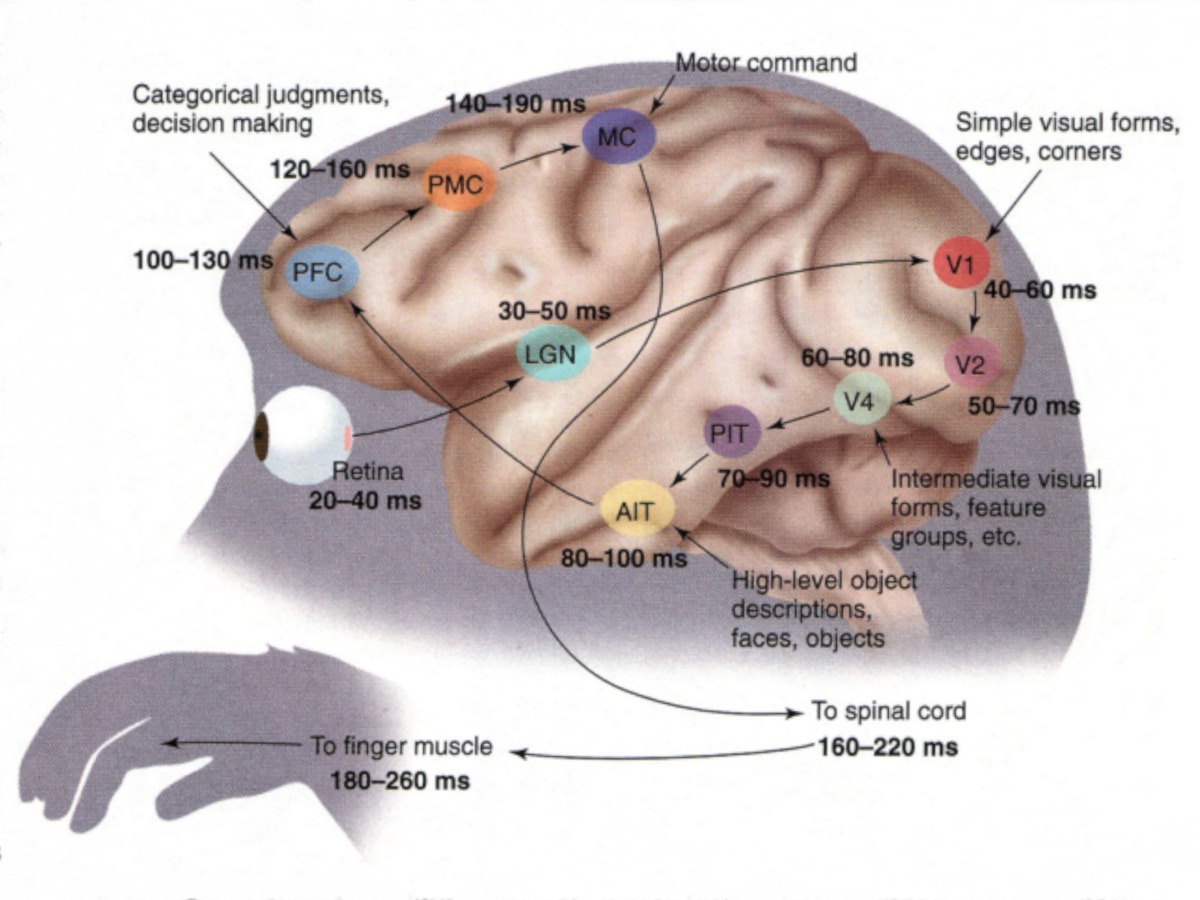
\includegraphics[width=.7\textwidth]{figures/visual-latency-estimate.jpg}
\caption{From~\citep{thorpe_seeking_2001} \note{get the rights or redo a schematics}}\label{fig:thorpe}
\end{figure}

\subsection{How timing encodes analogous profile}\label{how-timing-encodes-analogous-profile}
An important characteristic of neuronal information is that it consists mainly in the transfer of action potentials, or spikes, which consist of brief impulses that propagate along the axons of neurons. These have the particularity of being essentially binary in their amplitude (that is to say, they are prototypical, all or nothing). An important consequence of the speed of processing is that it implies that it is carried out using only very few spikes. Indeed, if we consider that a behavioral response in only 120 ms consists of about ten processing stages following the ``forward'' pathways of the visual system, then this imposes that the processing in a single area is performed with a reduced number of spikes. Neurophysiologists tipcally use firing sequences to characterize the activity of neurons using different statistics on their individual timing~\citep{perkel_neuronal_1967} but also the dependance across neurons~\citep{perkel_neuronal_1967-1}.

Numerous studies demonstrated the importance of precise timing in neural population activity~\citep{davis_spontaneous_2021}, efficient encoding thanks to the use of spike latencies~\citep{perrinet_coding_2004,gollisch_rapid_2008} or precise timing in the auditory system~\citep{deweese_binary_2003,carr_circuit_1990}. All these findings, and more~\citep{bohte_evidence_2004}, highlight the importance of the temporal aspect of the neural code and suggest the existence of repeated spatio-temporal patterns in the spike train. Note also that depending on how an in vitro cell is driven, this may influence the reliability of spike timing in neocortical neurons~\citep{mainen_reliability_1995}.

\begin{figure}
\centering
\note{redo a figure similar to the thorpe code}%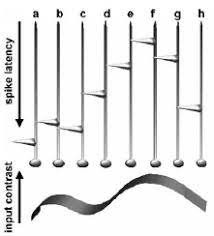
\includegraphics{images/roc.jpg}
\caption{Latency coding. An input analog profile is encoded in latencies: the higher the contrast, the shorter the latency. In this example, one generates at most one spike per neuron.
}\label{fig:roc}
\end{figure}

At the level of dynamic processing of visual information, it has been shown that an encoding of the values of luminance imminence in the image instead of the retina~\citep{gollisch_rapid_2008}. Notably one can appreciate in figure 1 that the response of ganglion cells to visual gratings that are flashed onto the retina. The authors showed that the neuronal response could be encoded in the latency of the response and not only in the frequency of discharge as is often assumed. In figure 4 of the same article, these results are extended to natural images and show a qualitatively similar behavior. The conclusion of the authors is that the discharge latency of the neurons allows to encode spatial characteristics of the image. First-spike latency codes are a feasible mechanism for information transfer even when biologically plausible estimates of stimulus onset are taken into account~\citep{chase_first-spike_2007}. Interestingly, such fine latency effect can be at the origin of somme visual illusions, for instance the illusion of false colors in the \href{https://michaelbach.de/ot/col-Benham/index.html}{Benham Top} based based on center-surround interactions in the parvocellular pathway~\citep{kenyon_theory_2004}.

Similar results have been demonstrated through neurophysiological recordings in the primary visual cortex and show that different levels of visual activity will induce different levels of neuronal discharge latency in the primary visual area~\citep{celebrini_dynamics_1993}. Many models have used these properties in temporal coding to build fast image categorization networks. These models take the form of artificial spiking neural networks (SNNs) and have been able to demonstrate their practical applications for image categorization~\citep{thorpe_speed_1996}. This work has been extended to include unsupervised learning capabilities and we have recently developed a SNN architecture that allows to categorize images of different classes in only a few spikes~\citep{grimaldi_homeostatic_2021,grimaldi_robust_2022}. This type of modeling is extremely important with respect to the development of a new generation of cameras called Silicon Cameras which, instead of using a basic frame-based representation, uses a representation similar to the one we have just described and which consists in representing the image by events~\citep{rasetto_challenges_2022}. This type of modeling often uses the classical architecture of image categorization developed in deep learning while adapting it to the specificity of the event-based representation~\citep{goltz_fast_2021}. Note also that timing is not entirely sensorial or internal but in~\citep{safaie_turning_2020}, they found that ``timing accuracy was improved when the environment afforded cues that rats can incorporate into motor routines. Timing, at least in animals, may thus be fundamentally embodied and situated.'' Altogether, these results show that ``that like other senses, vision relies heavily on temporal strategies and temporal neural codes to extract and represent spatial information''~\citep{rucci_temporal_2018}.

\section{Precise spike timings in neural assemblies}

\subsection{From synfire chains\ldots{}}\label{from-synfire-chains}
The analysis of generic raster plots reveals particular traits that hint at the role of a precise timing. For instance, the firing rate is highly irregular~\citep{softky_highly_1993}, which makes it inconsistent with temporal integration of random EPSPs. It has also been observed that the response of a neuron in a cortical slice to a current step could be highly non-reproducible, where the first spike is aligned but the subsequent spike times tend to diffuse for independent repetitions of the stimulation~\citep{mainen_reliability_1995} (see Figur
~\ref{fig:mainen}). When driven by a highly dynamic \emph{frozen} noise, the output spikes are highly reproducible. This is consistent with the differential role of different stimulus frequencies on the reliability of spike timing reported in~\citep{nowak_influence_1997} : ``we found that, as expected given the resistive and capacitive properties of cortical neurons, low frequencies have a larger effect on the membrane potential of cortical neurons than do higher frequencies. However, increasing the amount of gamma range fluctuations in a stimulus leads to more precise timing of action potentials.''

\begin{figure}
\centering
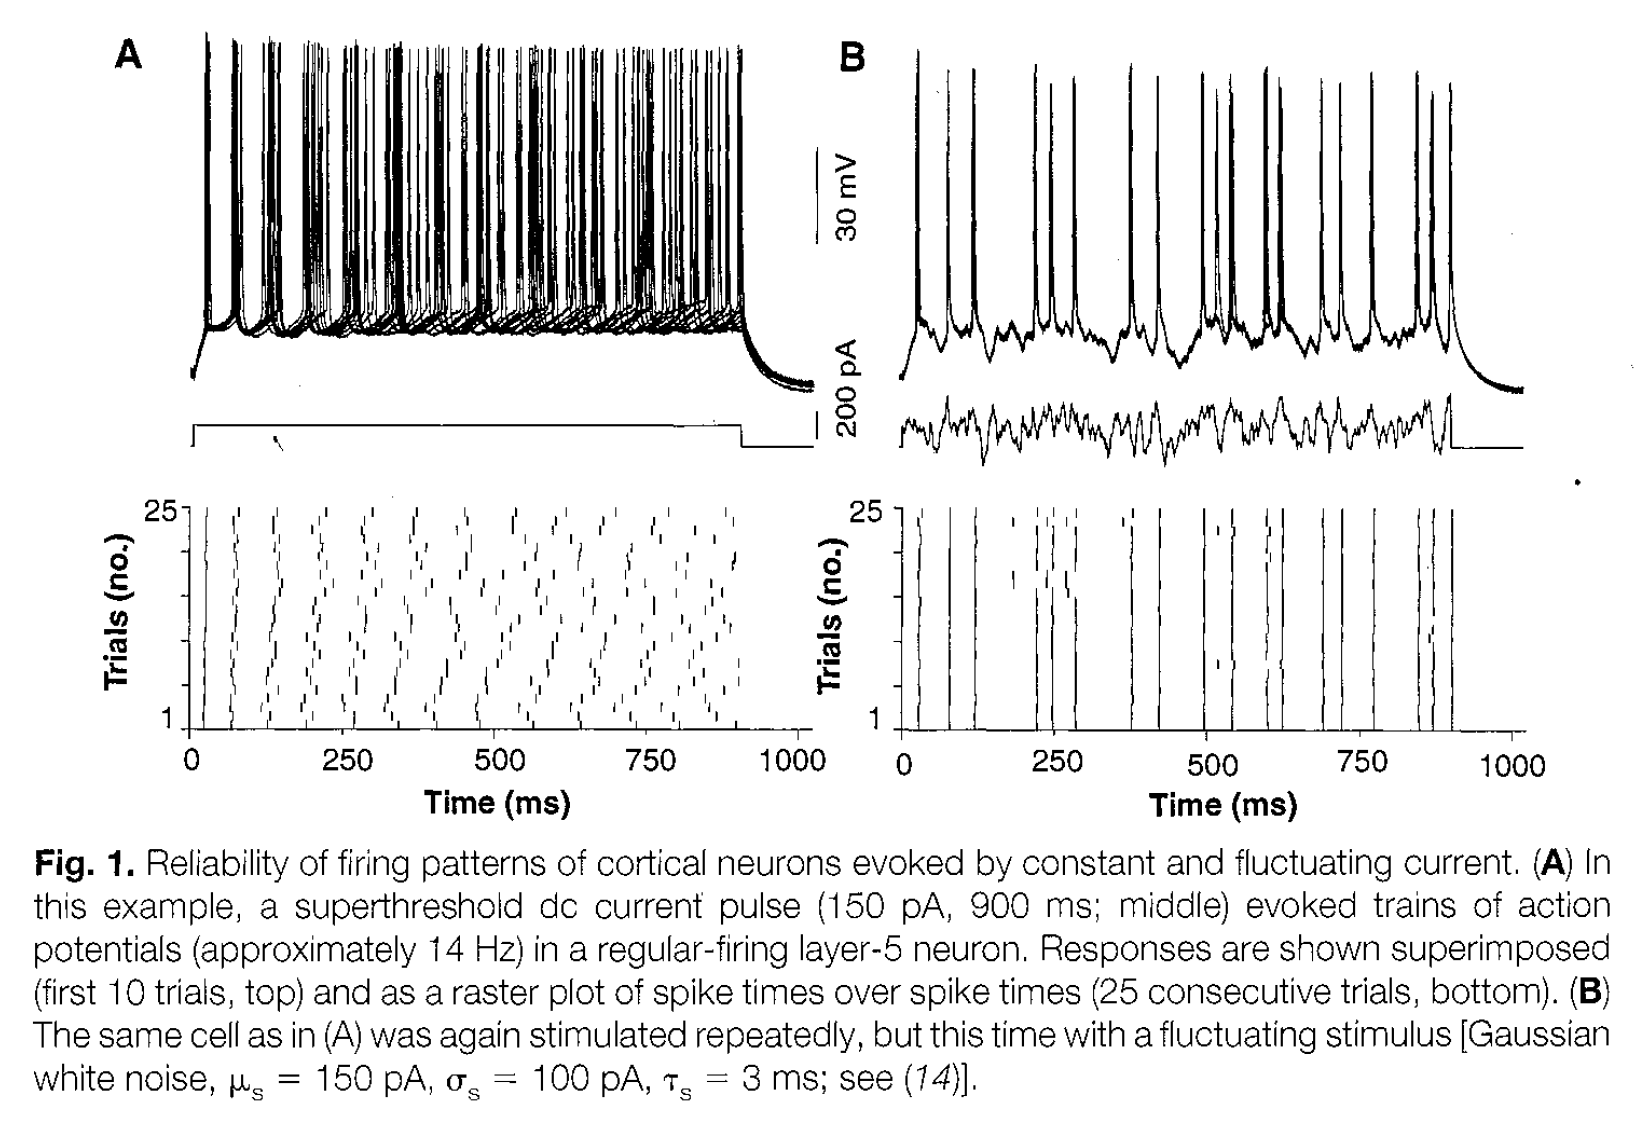
\includegraphics[width=.7\textwidth]{figures/MainenSejnowski1995.png} % TODO replace by the simulation
\caption{The timing of the spikes produced following the repetition of a step stimuli is less reproducible than that to a noisy stimulus. While this seems paradoxical at first sight, this is due to the use of the same \emph{frozen} noise at each repetition and highlight the highly reproducible pattern of spikes when it is driven by a highly dynamic input. See this \href{https://github.com/laurentperrinet/2022_UE-neurosciences-computationnelles/blob/master/C_MainenSejnowski1995.ipynb}{notebook} for a replication of this result using a simple LIF model.}\label{fig:mainen}
\end{figure}

In his book ``Corticonics''~\citep{abeles_corticonics_1991}, Moshe Abeles queried if the role of cortical neurons is whether to integrate synaptic inputs or rather to detect coincidences in temporal spiking patterns. The book gradually leads the reader from the macroscopic cortical anatomy and standard electrophysiological properties of single neurons to neural network models. While the first hypothesis favors the rate coding theory, the second possibility highlights the need for temporal precision in the neural code~\citep{paugam-moisy_computing_2012}. The book then demonstrates that this could take the form of ``synfire chains,'' that is synchronous activity on subsets of neurons which could be propagated in a stable fashion. Since this date, multiple experimental observations have suggested the existence of this precise zero-phase-lag spike synchronization in a defined subset of neurons~\citep{harris_organization_2003}.

It was shown that a simple model may allow the propagation of such synfire chains~\citep{gewaltig_propagation_1970}. This model considers the dynamics of leaky integrate-of-fire neurons in different groups of similar size. Each neuron of one group is connected by an excitatory synapse to the next. When a pulse is elicited in the first group, this may generate a spike in the next group. Depending on the weight value, this new activity may get more or less synchronized than the previous pulse (as measured by the standard deviation of spike times in the pulse). Recursively applying this to a sequence of groups generates either a synfire propagation or not. A simple simulation is shown in Figure
~\ref{fig:diesman}. A crucial aspect of this emergence is in particular the balance between excitation and inhibition~\citep{azouz_stimulus-selective_2008}. This was for instance modeled by feed-forward inhibition which is a fine-scaled latency mechanism that is an essential ingredient in modelling push-pull effects in the primary visual cortex~\citep{kremkow_push-pull_2016}.

\begin{figure}
\centering
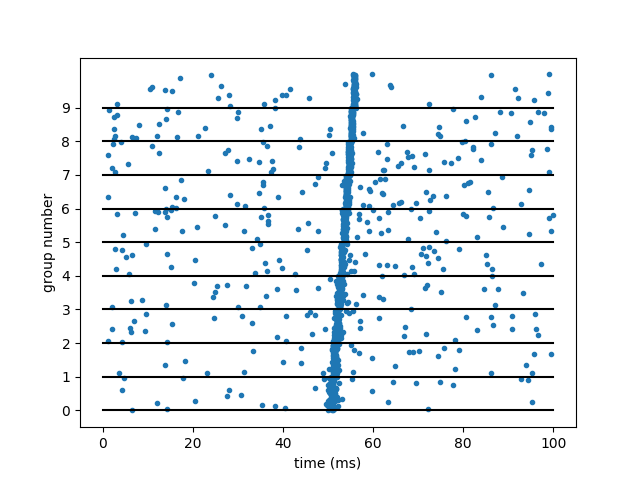
\includegraphics{figures/Diesmann_et_al_1999.png}
\caption{Simulation of a synfire propagation \href{https://brian2.readthedocs.io/en/stable/examples/frompapers.Diesmann_et_al_1999.html}{using Brian}. The model consists of 10 groups of 100 neurons each. A pulse with a given jitter is generated in the first group which here generates a pulse after a certain processing delay in the second group with a lower jitter. This allows the propagation of the synchronous activity along the chain of the neural groups.}\label{fig:diesman}
\end{figure}

Attempts have been made to detect such synfire chains in neurobiological data~\citep{schrader_detecting_2008}: ``The sensitivity is high enough to detect synfire chain activity in simultaneous single-unit recordings of 100 to 200 neurons from such data, enabling application to experimental data in the near future.'' Further models have shown that such synfire chains could be embedded in topographies~\citep{aviel_embedding_2003} or using conductance-based neurons with feed-forward inhibition to improve the robustness of the propagation~\citep{kremkow_functional_2010}. In particular, this was implemented using the pyNN language~\citep{davison_pynn_2008} both in CPU-based and neuromorphic hardware~\citep{pfeil_six_2013} (see Figure~\ref{fig:pynn}).

\begin{figure}
\centering
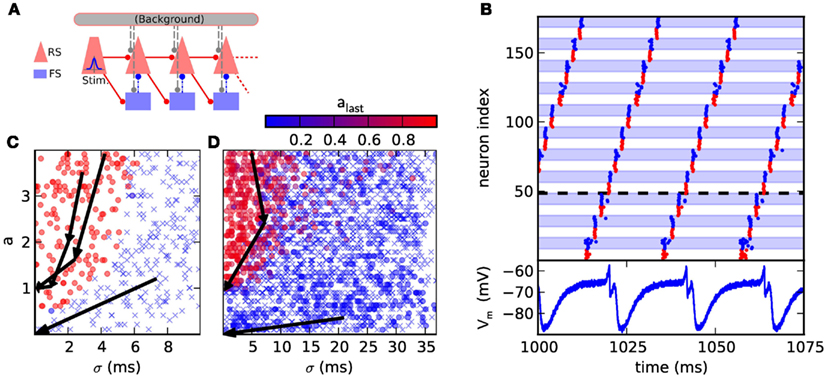
\includegraphics{figures/fnins-07-00011-g004.jpg}
\caption{A pyNN implementation of a Synfire chain with feedforward inhibition. The background is only utilized in the original model, where it is implemented as random Gaussian current. For the presented hardware implementation it has been omitted due to network size constraints. As compensation for missing background stimuli, the resting potential was increased to ensure a comparable excitability of the neurons. The state space gives the duration of synfire chains as a function of the protocol's parameters and compares (C) CPU to (D) neuromorphic implementations.}\label{fig:pynn}
\end{figure}

Note also that synchronicity may explain some unintuitive results. Indeed it has been shown that thalamocortical synapses are relatively weak compared to the amount of intra-cortical activity. However, this pathway is sufficient to drive the cortex as this input is more often synchronously active~\citep{bruno_cortex_2006}.

Some experimental results show the emergence of synchrony, for instance in motor cortical function~\citep{riehle_spike_1997}. Interestingly, authors showed that ``Accurate spike synchronization occurred in relation to external events (stimuli, movements) and was commonly accompanied by discharge rate modulations but without precise time locking of the spikes to these external events. Spike synchronization also occurred in relation to purely internal events (stimulus expectancy), where firing rate modulations were distinctly absent. These findings indicate that internally generated synchronization of individual spike discharges may subserve the cortical organization of cognitive motor processes.'' Moreover, such emergence could change over the learning period involved in learning a task~\citep{kilavik_long-term_2009} and showed some tuning to to movement direction and reaction time~\citep{grammont_spike_2003}. It is important to note that synchronous events tended to lock to LFP beta waves~\citep{denker_lfp_2018}, and was extended to larger assemblies~\citep{torre_synchronous_2016} using statistical methods (see~\ref{sec:detection}).

In~\citep{brette_computing_2012}, the author proposes a simple spike-based computational framework, based on the idea that stimulus-induced synchrony can be used to extract sensory invariants (for example, the location of a sound source), which is a difficult task for classical neural networks. It relies on the simple remark that a series of repeated coincidences is in itself an invariant. Many aspects of perception rely on extracting invariant features, such as the spatial location of a time-varying sound, the identity of an odor with fluctuating intensity, the pitch of a musical note.

\subsubsection{.. to traveling waves \ldots{}}\label{to-traveling-waves}
TODO :~\citep{bringuier_horizontal_1999} latency basin

Statistical dependencies in the responses of sensory neurons govern both the amount of stimulus information conveyed and the means by which downstream neurons can extract it. This is put in evidence by analysing the functional significance of correlated firing in a complete population of macaque parasol retinal ganglion cells using a model of multi-neuron spike responses~\citep{pillow_spatio-temporal_2008}. This show precise spatio-temporal differences in this recurrently connected assembly. The different aspects of information in the data are evaluated by a decoding strategy highlighting the role of correlations. A similar dataset used in~\citep{schneidman_weak_2006} is available from M. Berry's lab~\citep{berry_spike_2022}.

Propagating waves occur in many excitable media and were recently found in neural systems from retina to neocortex. While propagating waves are clearly present under anaesthesia, whether they also appear during awake and conscious states remains unclear. One possibility is that these waves are systematically missed in trial-averaged data, due to variability. A recent work~\citep{muller_stimulus-evoked_2014} presents a method for detecting propagating waves in noisy multichannel recordings. Applying this method to single-trial voltage-sensitive dye imaging data, they show that the stimulus-evoked population response in primary visual cortex of the awake monkey propagates as a travelling wave, with consistent dynamics across trials. A network model suggests that this reliability is the hallmark of the horizontal fibre network of superficial cortical layers. Propagating waves with similar properties occur independently in secondary visual cortex, but maintain precise phase relations with the waves in primary visual cortex. These results show that, in response to a visual stimulus, propagating waves are systematically evoked in several visual areas, generating a consistent spatiotemporal frame for further neuronal interactions.

\begin{figure}
\centering
%\includegraphics[width=1\textwidth,height=\textheight]{https://media.springernature.com/lw685/springer-static/image/art\%3A10.1038\%2Fs41467-021-26175-1/MediaObjects/41467_2021_26175_Fig1_HTML.png}
\caption{a Spike raster for repeated presentations (%N = 40) of a high-contrast (10\% Michelson contrast) drifting Gabor recorded from area MT of a fixating marmoset (stimulus-onset, red line; mean response, blue line). A single-trial LFP trace is plotted in gray, and the average LFP response is plotted in black. The relative power between baseline (−200 ms to stimulus-onset) and evoked fluctuations (stimulus-onset + 50--250 ms) significantly favored the evoked response (right panel; N = 110 trials; median = 1.89 dB, p = 0.000019, two-tailed Wilcoxon's ranked-sum test). b Same as in (a), but for a low contrast stimulus (2\% Michelson contrast). The relative power between baseline and evoked LFP fluctuations was not statistically different from parity (median = 1.23 dB, p = 0.087 two-tailed Wilcoxon's ranked-sum test). c An example of spontaneous LFP fluctuations structured as a traveling wave recorded from a spatially distributed multielectrode array in marmoset area MT. d Histogram of spontaneous spike probability as a function of the generalized phase of the LFP during fixation. e The average evoked response to low contrast stimuli was stronger when a more excitable phase (+ / - \pi rad) of a spontaneous traveling wave aligned with the retinotopic location of the target (aligned, green line) as compared to when a less excitable phase (0 rad) was aligned (unaligned, purple line; N = 43 wave and non-wave trials; shaded region SEM; p = 0.0000015 two-tailed Wilcoxon's rank-sum test). Data for panels c--e modified from Davis et al.17 with permission.
}\label{fig:davis}
\end{figure}

More recently Advanced recording techniques have enabled the identification of travelling waves of neuronal activity in different areas of the cortex~\citep{muller_cortical_2018}. Authors review these findings, consider the mechanisms by which travelling waves are generated and evaluate their possible roles in cortical function. In particular, spontaneous traveling waves naturally emerge from horizontal fiber time delays and travel through locally asynchronous-irregular states~\citep{davis_spontaneous_2021}. Studies of sensory-evoked neuronal responses often focus on mean spike rates, with fluctuations treated as internally-generated noise. However, fluctuations of spontaneous activity, often organized as traveling waves, shape stimulus-evoked responses and perceptual sensitivity. The mechanisms underlying these waves are unknown. Further, it is unclear whether waves are consistent with the low rate and weakly correlated ``asynchronous-irregular'' dynamics observed in cortical recordings. Here, authors describe a large-scale computational model with topographically-organized connectivity and conduction delays relevant to biological scales. They find that spontaneous traveling waves are a general property of these networks. The traveling waves that occur in the model are sparse, with only a small fraction of neurons participating in any individual wave. Consequently, they do not induce measurable spike correlations and remain consistent with locally asynchronous irregular states. Further, by modulating local network state, they can shape responses to incoming inputs as observed in vivo.

~\citep{linden_movement_2021} present ensemble-recordings of neurons in the lumbar spinal cord that indicate that, rather than alternating, the population is performing a low-dimensional ``rotation'' in neural space, in which the neural activity is cycling through all phases continuously during the rhythmic behavior.

\subsubsection{Spike Synchronization and Rate Modulation Differentially Involved in Motor Cortical Function~\citep{riehle_spike_1997}}\label{spike-synchronization-and-rate-modulation-differentially-involved-in-motor-cortical-function-doi10.1126science.278.5345.1950}
It is now commonly accepted that planning and execution of movements are based on distributed processing by neuronal populations in motor cortical areas~\citep{grammont_precise_1999}. It is less clear, though, how these populations organize dynamically to cope with the momentary computational demands. Simultaneously recorded activities of neurons in the primary motor cortex of monkeys during performance of a delayed-pointing task exhibited context-dependent, rapid changes in the patterns of coincident action potentials. Accurate spike synchronization occurred in relation to external events (stimuli, movements) and was commonly accompanied by discharge rate modulations but without precise time locking of the spikes to these external events. Spike synchronization also occurred in relation to purely internal events (stimulus expectancy), where firing rate modulations were distinctly absent. These findings indicate that internally generated synchronization of individual spike discharges may subserve the cortical organization of cognitive motor processes.

~\citep{chemla_suppressive_2019}

\subsubsection{TODO \ldots{} and to synfire braids and polychronous groups}\label{todo-and-to-synfire-braids-and-polychronous-groups}
\begin{itemize}
 \item
 ~\citep{bienenstock_model_1995} : from synfire chains to Synfire braids
\end{itemize}

In neuronal models, an efficient use or detection of these spatio-temporal patterns embedded in the spike train comes with the integration of heterogeneous delays~\citep{guise_bayesian_2014,zhang_supervised_2020}. Notably, Izhikevich~\citep{izhikevich_polychronization_2006} introduced the notion of polychronous groups (PGs) as a repetitive motif of spikes defined by a subset of neurons with different, yet precise, spiking delays. This representation has a much greater information capacity in comparison to other neural coding approaches through their connectivity and the possible coexistence of numerous superposed PGs.

sparse in time and space : AL Barth and JF Poulet Trends in Neurosciences 35.6 (2012), pp.~345-355. 
CC Petersen and S Crochet, Neuron 78.1 (2013), pp.~28-48.

\begin{itemize}
\item
  recent theories of binding by synchrony : Fries 2005 trends cog neuro with spikes arriving at peak susceptibility (top of a cycle) or down, van Rullen, Laura Dugué
\item
  cell assembly hypothesis: neurons coordinate their activity through the formation and repetitive co-activation of groups. https://link-springer-com.insb.bib.cnrs.fr/article/10.1007/s10827-021-00801-9 Hebb DO. The organisation of behaviour: a neuropsychological theory. New York: Science Editions; 1949.
\item
  A notable exception is the polychronization model of Izhikevich~\citep{izhikevich_polychronization_2006}, which combined the construction of a random recurrent model of spiking neurons including such delays and whose weights evolved with a Spike-Time Dependent Plasticity (STDP) learning rule. In this model, raster plot analysis showed repeated activation of Polychronous Groups (PGs), i.e., specific spike patterns with a specific sequence of activations.
\end{itemize}

\subsection{Are there precise heterosynaptic spiking motifs in the brain?}\label{are-there-precise-heterosynaptic-spiking-motifs-in-the-brain}
Currently, there is a consensus for rate-based coding models in computational and biological neuroscience. Nevertheless, there is a substantial literature in neurobiology indicating that brain dynamics often organize into stereotyped sequences (like synfire chains~\citep{ikegaya_synfire_2004}, packets~\citep{luczak_sequential_2007} or hippocampal sequences~\citep{pastalkova_internally_2008,villette_internally_2015} and on the role of such precise spike timing in downstream information transfer and coding~\citep{villette_internally_2015,branco_dendritic_2010,luczak_packet-based_2015}. This is for instance relevant in sensory pathways in vision~\citep{meister_concerted_1995}, audition~\citep{decharms_primary_1996}, olfaction~\citep{wehr_odour_1996} or touch~\citep{johansson_first_2004}. In particular, one theoretical viewpoint considers synfire braids (Bienenstock, 1995), where a precise sequential motif of spikes will synchronize as it reaches the soma of a neuron for which synaptic delays are adequately tuned. In particular, computational modeling shows that at the scale of neurons, an efficient neural code can emerge where spike times are organized in prototypical, precise temporal motifs (Izhikevich, 2006) which he defined as polychronous groups.

Stereotyped sequences of neuronal activation have been particularly well described in the adult hippocampus and related to its function in mental travel in time and space~\citep{buzsaki_space_2018}. These sequences can be internally generated~\citep{pastalkova_internally_2008,villette_internally_2015} and are formed by the chained activation of orthogonal assemblies, themselves organized as sequence packets (Malvache et al., 2016). Thus, hippocampal sequences are formed by the ordered activation of smaller sequence motifs. They are stereotyped and robust, since neurons can be activated in the same order across days (see Figure
~\ref{fig:haimerl} from~\citep{haimerl_internal_2019} below). As a consequence, hippocampal sequences may rely on an internally hardwired structure and form the functional building blocks for encoding, storing and retrieving experience.

\begin{figure}
\centering
%\includegraphics{https://www.pnas.org/cms/10.1073/pnas.1718518116/asset/ab9a48f6-b28f-40c1-978e-6f6dbec39b98/assets/graphic/pnas.1718518116fig01.jpeg}
\caption{Mixed distance and duration representation in CA1. (A) Calcium fluorescence (heatmap) of CA1 neurons participating to run sequences in consecutive imaging sessions. Cells have been selected and ordered with respect to their activity in the first imaging session (Top). The black line represents speed of the mouse.}\label{fig:haimerl}
\end{figure}

TODO: read~\citep{luczak_packet-based_2015} Luczak A, McNaughton BL, Harris KD. Packet-based communication in the cortex. Nat Rev Neurosci. 2015;16(12):745--55.

In~\citep{van_kempen_top-down_2021}, it was shown that attentional information from V4 or arousal can change the timings of groups of events in V1. They develop a HMM model for quantifying the transitions. ``In this study, van Kempen et al.~show that fluctuations in neural excitability are coordinated between visual areas with retinotopic precision. Top-down attention drives interareal coordination along the reverse cortical hierarchy, predicting better behavioral performance with increased coordination.''

\subsection{Cortical songs}\label{cortical-songs}
\begin{itemize}
 \item
  Ikegaya and colleagues~\citep{ikegaya_synfire_2004} worked on spontaneous activity in vitro and in vivo. They demonstrated that in cortical activity, we can find a repetition of several motifs. In PSCs, but also in spike activity. These sequences repeat after minutes and have a precise spatio temporal structure with a ms precision. They can be specific of a particular layer or colomn, are synchronized with network activity oscillation and can involve several cells. They also demonstated that these sequences can form supersequences : the cortical songs. It consist of the assembly of several sequences which repeat in a specific order with a compressed timing.
\item
  ``We find precise repetitions of spontaneous patterns of synaptic inputs in neocortical neurons in vivo and in vitro. These patterns repeat after minutes, maintaining millisecond accuracy.''
\item
  Precisely repeating motifs of spontaneous synaptic activity in slices: duration around 1s +/- .5 s. Some events in motifs are of similar size but sometimes absent - better described by Bernouilli than SE (and covariance)
\item
  \emph{in vivo} spontaneous activity also reveals repeating sequences. About 3000 sequences, each involving 3-10 cells out of about 900, and last up to 3 seconds
\item
  topography: ``Sequences had specific topographic structures, in some cases involving only a particular layer or a vertical column of cells or cells located in a cluster (Fig. 4, A and B, and fig.~S3B). (\ldots) Therefore, repeating temporal patterns of activation (\ldots) were associated with a structured spatial organization of the neurons that formed them.''
\item
  ``Cortical songs: modular assemblies of repeated sequences'': hierarchical detection.
\item
  in cotical songs, there is a ``compressing timing'' which may be taken into account by a similar mechanism as maxpooling in CNNs for space, but in time. Or there may be a mechanism for controlling the replay speed (pulvinar, \ldots{} , ?)
\end{itemize}

\begin{figure}
\centering
%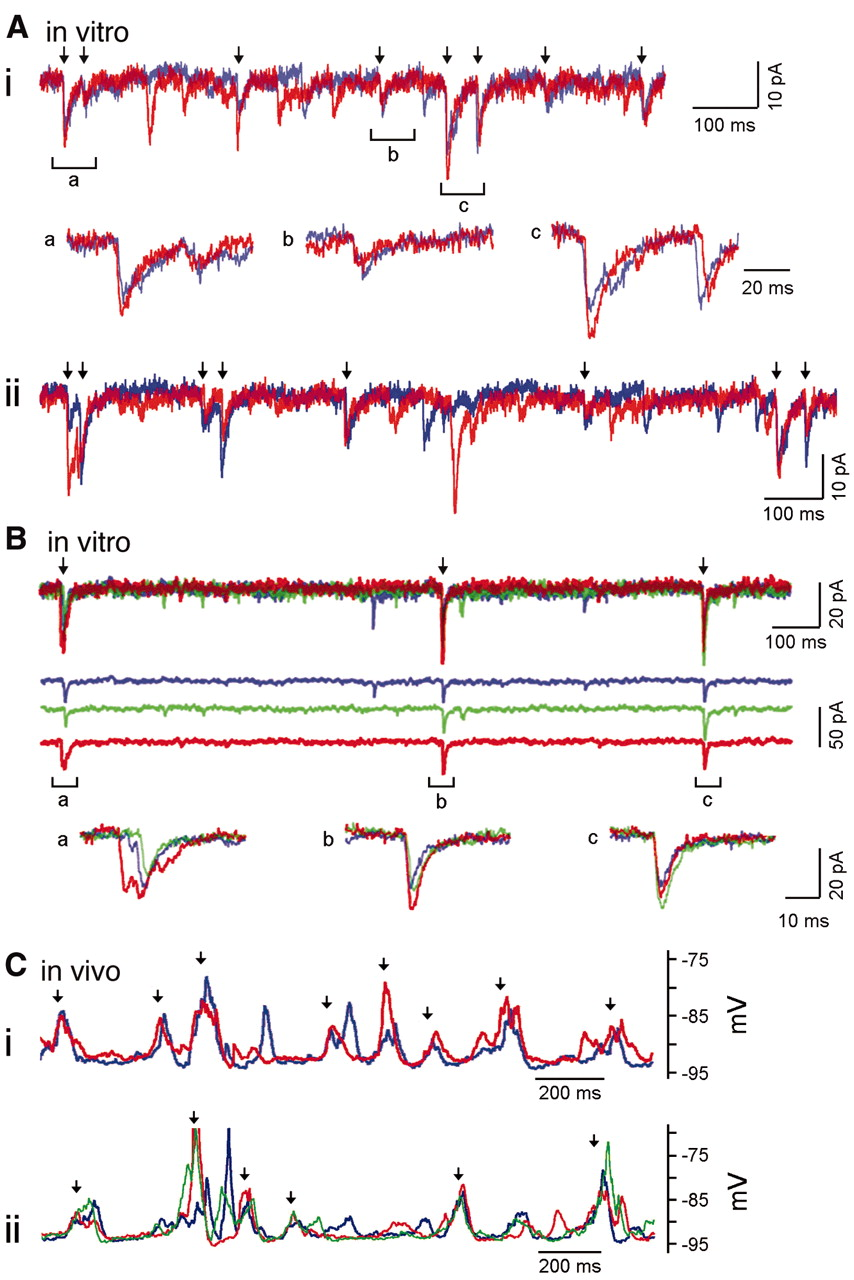
\includegraphics{figures/Ikegaya2004zse0150424620001.jpeg}
\caption{Fig. 1. from~\citep{ikegaya_synfire_2004} Repeated motifs of spontaneous synaptic activity in vitro and in vivo. (A) Repeated motifs of intracellular activity from layer 5 pyramidal neurons in slices. Panels show segments (red) of the same voltage-clamp recording from the same cell repeating seconds or minutes after the initial occurrence (blue). Arrows indicate timings of repeated PSCs. (i) Upper trace: low--temporal resolution display of spontaneous activity of a neuron. Lower traces: higher resolution display of the repeated motif at indicated regions of the trace (a to c). (ii) Example of a longer motif. (B) Three repetitions of a motif. The top traces show the motifs superimposed on each other (blue, green, and red), the middle traces show these same traces individually, and the bottom traces show temporally magnified regions of the motifs (a to c). (C) Repeated sequences of intracellular current-clamp recordings in vivo. Two (i) and three (ii) repetitions of motifs are shown. Shuffle tests were performed on traces (i), a to c, yielding significantly fewer repeats (fig.~S2, P  0.02). In (i), the blue trace is shifted --2.75 mV; in (ii), the blue trace is shifted --1.58 mV, and the green +0.79 mV.}\label{fig:Ikegaya2004}
\end{figure}

It is interesting to make a parallel with the ``Rapid Formation of Robust Auditory Memories'' reported in~\citep{agus_rapid_2010} which uses noise patterns. They " used random waveforms to probe the formation of new memories for arbitrary complex sounds. A behavioral measure was designed, based on the detection of repetitions embedded in noises up to 4 s long." The task is to detect the repetition of the same (frozen) noise within a trial. " Unbeknownst to listeners, some noise samples reoccurred randomly throughout an experimental block." they showed that the ``repeated exposure induced learning for otherwise totally unpredictable and meaningless sounds'' by showing that the sensitivity increases in that case. Note that ``acoustical analyses failed to reveal any obvious differences between good and bad noises'' and that ``Time reversal had no significant effect on the RefRN advantage'' (quite surprising). The Learning is unsupervised (statistical, automatic), fast-acting (phase transition, ``insight''), and long-lasting (memorization).

Such observations suggest that neuronal groups or ensembles, rather than individual neurons, are emergent functional units of cortical activity~\citep{miller_visual_2014}. This work shows, using two-photon calcium imaging of populations of neurons from the primary visual cortex of awake mice during visual stimulation and spontaneous activity, that whereas intrinsic ensembles recur at random time intervals, visually evoked ensembles are time-locked to stimuli. It proposes that visual stimuli recruit endogenously generated ensembles to represent visual attributes. Note that evoked ensembles in response to a natural movie played in a loop were precisely timed across repetitions (Fig. 7).

\subsection{outline}\label{outline}
A natural candidate to use these precise temporal patterns in the brain is to use Spiking Neural Networks (SNNs)~\citep{maass_networks_1997}. The approach which is at present most prominent in the SNNs community is to use existing algorithms from machine learning and to adapt them to the specificity of spiking architectures. One such example is to adapt the successes of deep learning algorithms and to transfer the back-propagation algorithm to SNNs, for instance with a surrogate gradient. This approach is quite successful, and SNNs approach in some case the performance of Deep Learning algorithms, for instance on the N-MNIST dataset for categorizing digits in a stream of events. However, most biological neural systems use spikes and are obviously more efficient than current state-of-the-art vision systems, both in terms of efficiency (accuracy), in speed (latency), and energy consumption. There is therefore an immense gap in the way we understand biology to translate it to the efficiency of SNNs. Our approach will be to focus on the temporal representation of information directly. In particular, our objective is to fully exploit the capacity of spiking neurons to detect synchronous patterns.

\textbf{TODO: a paragraph on our existing work}
Our approach would be distinct than these approaches from us and colleagues as we will directly deal with delays in the system at the presynaptic level.

there are temporal delays in the nervous system, both at the neural~\citep{perrinet_active_2014} and behavioral~\citep{khoei_flash-lag_2017} levels. Extending this knowledge to the optimization of delays in a SNN will provide a breakthrough in the efficiency of these networks.

may be used for motion detection and interpolation~\citep{kaplan_anisotropic_2013}~\citep{khoei_flash-lag_2017}


Remarkably, novel neuromorphic chips use a representation similar to that of real neurons~\citep{rasetto_challenges_2022}. For example, event-based cameras provide a stream of binary asynchronous events signaling detectable changes in luminance, and information is represented by these spike-based temporal motifs, hence their name ``silicon retinas'' (see Figure \ref{fig:silicon_retina}). For such devices, it is crucial to better understand the potential of using such event-based representations in order to devise novel algorithms.

\begin{figure}
\centering
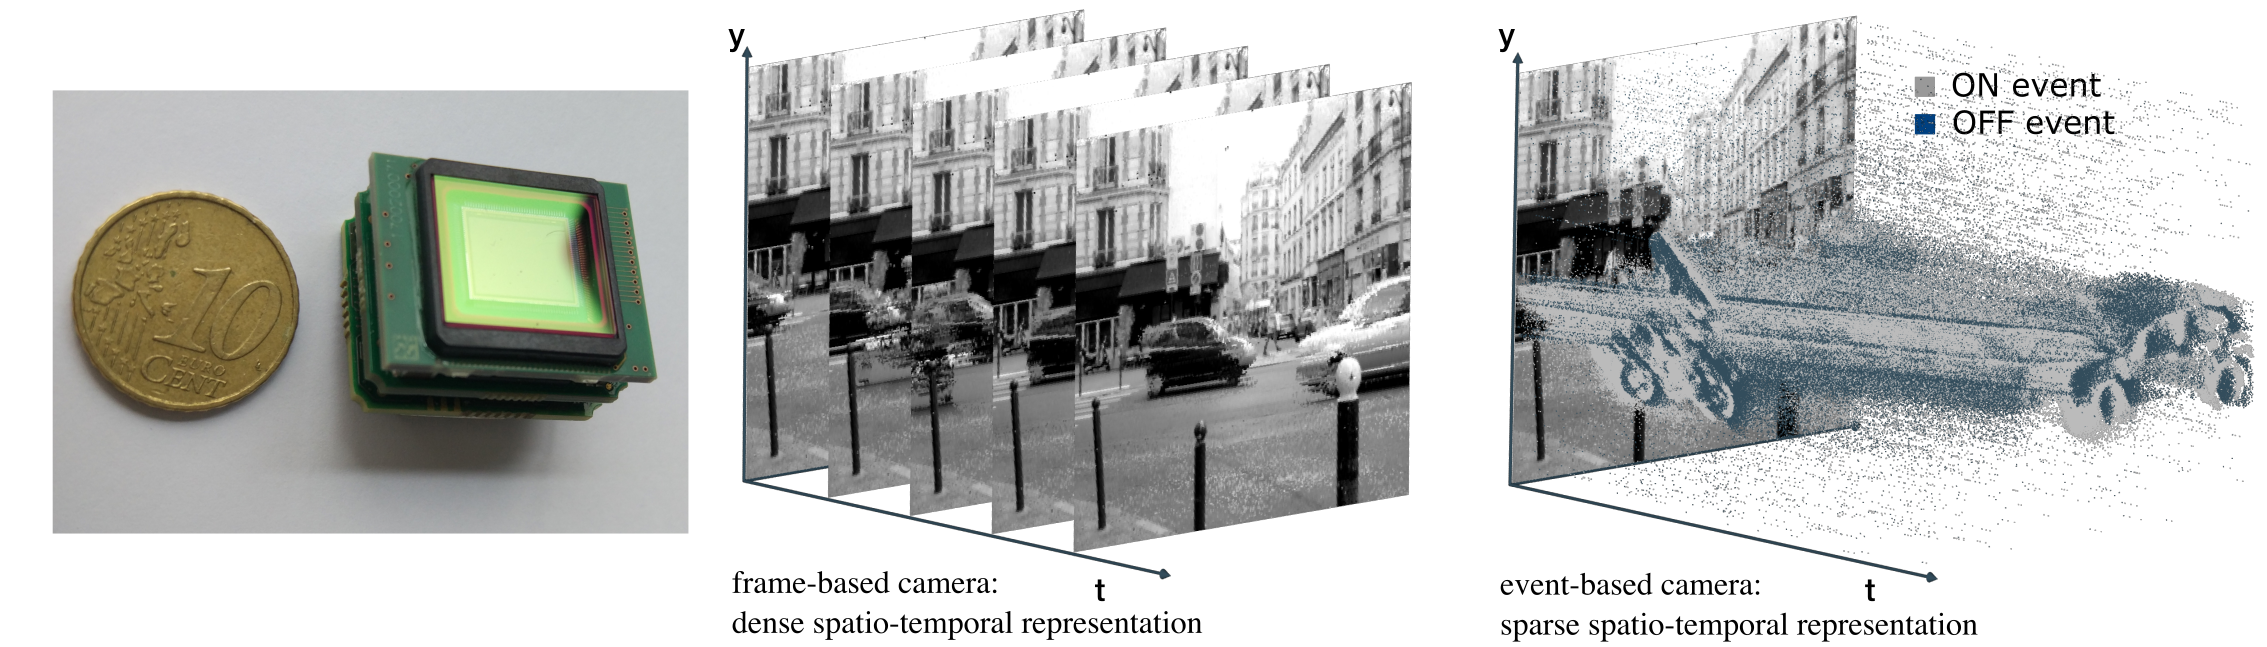
\includegraphics{figures/event_driven_computations.png}
\caption{A miniature, event-based ATIS sensor. Contrary to a classical frame-based camera for which a full dense image representation is given at discrete, regularly spaced timings, the event-based camera provides with events at the micro-second resolution. These are sparse as they represent luminance increments or decrements (ON and OFF events, respectively).}\label{fig:silicon_retina}
\end{figure}

This section has provided evidence that polychronous groups are an important apsect of information representation in biology with important application in data analysis and neuromorphic engineering. The rest of this review paper is organized as follows.

First, we will review models for the detection of polychronous groups:

\begin{itemize}
\item
  A crucial advantage of Spiking Neural Networks (SNNs) architectures lies in its processing of temporal information. Yet, most SNNs encode the temporal signal as an analog signal and try to ``cross-compile'' classical Neural Network to a spiking architecture. To go beyond the state-of-the-art, we will review here on one core computation of a spiking neuron, that is, is its ability to switch from the classical integrator mode (summing analog currents on its synapses) to a synchrony detector where it emits a spike whenever presynaptic spiking inputs are synchronized. To overcome the diversity of input presynaptic patterns, we will explore different existing architectures to learn to detect stable ``polychronous`` events, that is, volleys of spikes which are stable up to certain synaptic delays. These models will be compared in light of neuroscientific and computational perspectives. We review theoretical and computational foundations of PG detection in models.
\item
  Application to Image processing using sparse spiking representations: Using the core computational unit defined, extension of the computation to a topographic representation similar to that observed in the primary visual cortex of mammals. design of micro-circuits with specific lateral interactions will allow us to design efficient micro-circuits for the sparse representation of images.
\end{itemize}

Finally we will discuss future avenues for effective PG detection and learning in event streams.

\section{Models for the detection of precise heterosynaptic spiking motifs}\label{sec:detection}

A popular model for the detection of latency patterns is the tempotron~\citep{gutig_tempotron_2006}. This model is in particular reviewed in~\citep{gutig_spike_2014}. The Tempotron is a supervised synaptic learning algorithm which classifies a distractor from a target motif. This aims at extending the perceptron which does not incorporate a spike timing framework. The tempotron learning rule is derived by an optimization process and takes the form of a STDP rule. It is general consensus that spike timing (STDP) plays a crucial role in the development of synaptic efficacy for many different kinds of neurons~\citep{caporale_spike_2008}. The limits of this model is that it's output is only binary and that it's storage capacity are limited.

Some other models of latency motifs detection using STDP learning rules. For instance,~\citep{kheradpisheh_stdp-based_2018} implements a STDP-based spiking deep convolutional neural networks for object recognition;~\citep{tavanaei_representation_2018} develops a form of spike-based, competitive learning applied for unsupervised learning. In~\citep{russo_cell_2017}, authors developed novel machine learning tools and statistical tests for unsupervised spatio-temporal pattern detection in non-stationary environments, which was applied to simultaneous electrophysiological recordings from tens to hundreds of neurons for decoding cognitive processes from neural activity.

In the following of this section, we will review theoretical models which directly tackle the problem of using precise heterosynaptic spiking motifs.

\subsection{Izhikevitch's polychronization model}\label{izhikevitchs-polychronization-model}
Considering the number of spikes required to exceed a voltage threshold, asynchronous signals are less efficient than synchronous signals. However, taking axonal propagation times into account, synchronous signals may not coincide significantly at the post-synaptic neuron contrary to asynchronous or polychronous signals. The term polychronous was first introduced in 2006, by E. Izhichevitch in~\citep{izhikevich_polychronization_2006}. He defines this term after pointing out a particular organization of the neurons of his spiking artificial neural network. The network is characterized by a timing-dependant learning rule for weights (STDP) and by fixed conduction delays between neurons. Due to the interplay between the delays and STDP, the spiking neurons spontaneously self-organize into groups and generate patterns of stereotypical polychronous activity, i.e.~exhibit reproducible time-locked but not synchronous firing patterns. The neurons composing a group discharge at different times, but due to delays, the spikes reach the postsynaptic neuron at the same time. This synchrony leads to the summation of the excitatory post-synaptic potentials evoked by each spike and thus to the crossing of the voltage threshold and to the discharge of a spike. According to the STDP rule, the neurons involved in this activity will see their weight of synaptic connection increase and thus, constitute a polychronous group. Interestingly, thanks to the fact that a neuron can be involved in different polychronous groups, the number of coexisting polychronous groups far exceeds the number of neurons in the network, resulting in an unprecedented memory capacity of the system.

This paper proposes a supervised delay learning algorithm for spiking neurons with temporal encoding, in which both the weight and delay of a synaptic connection can be adjusted to enhance the learning performance~\citep{wang}.

\begin{figure}
\centering
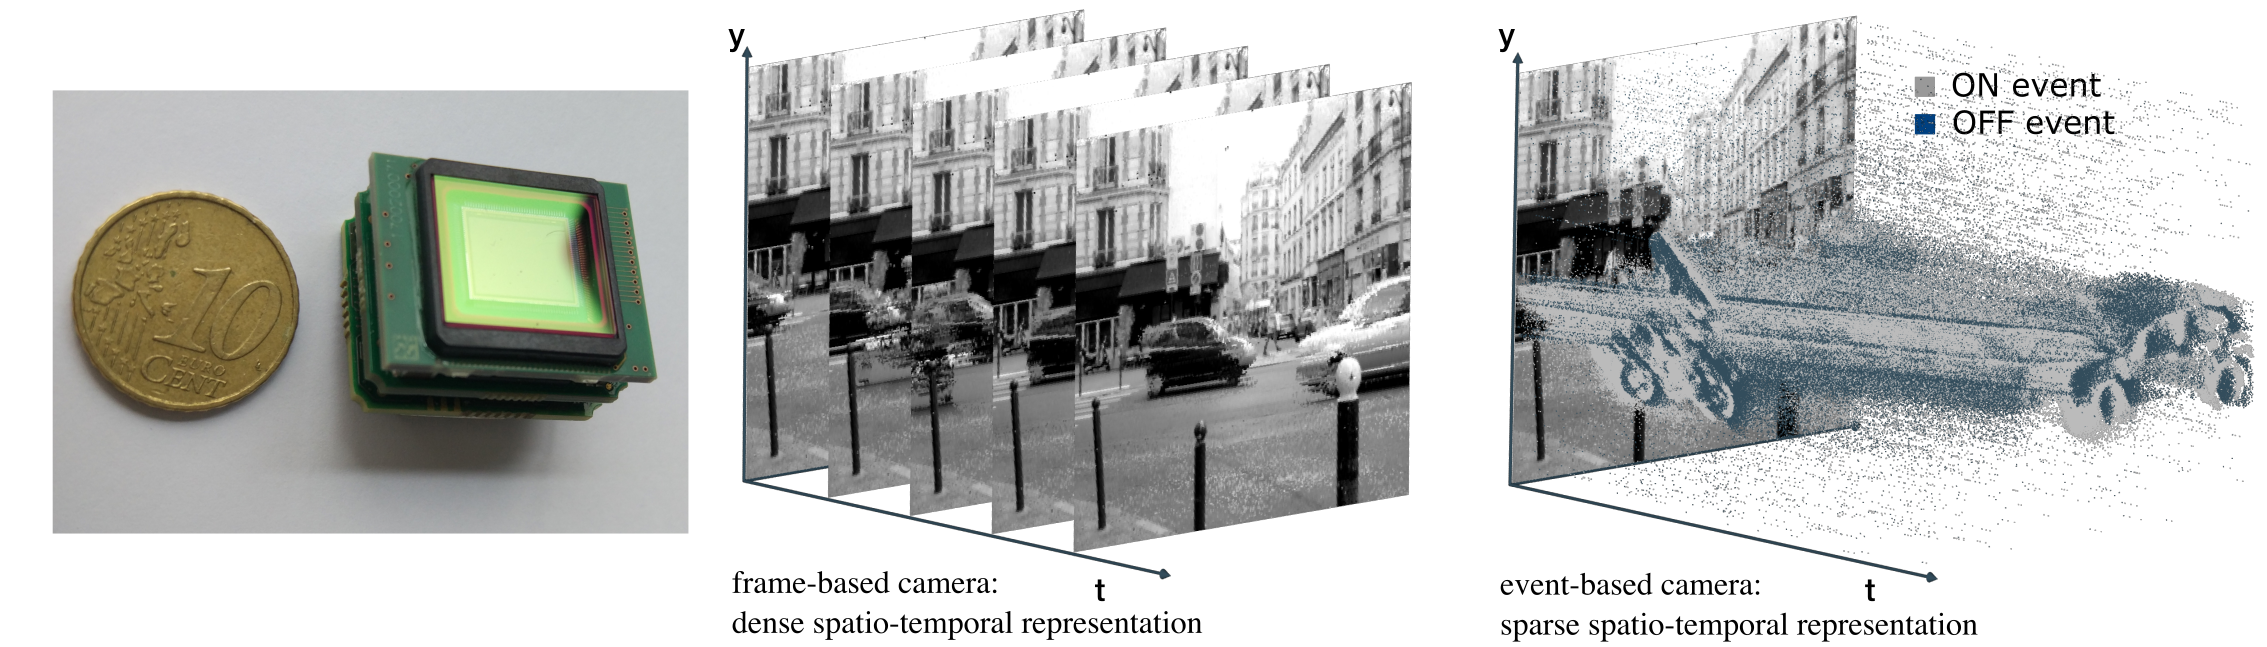
\includegraphics{figures/event_driven_computations.png}
\caption{\note{insert fig 2 of~\citep{izhikevich_polychronization_2006}}.}\label{fig:PG}
\end{figure}


Thus, the learning of delays allowing this polychronous group organization may be useful to detect temporal sequences of interest.

\begin{itemize}
\item
  Reproducing Polychronization: A Guide to Maximizing the Reproducibility of Spiking Network Models \url{https://www.frontiersin.org/articles/10.3389/fninf.2018.00046/full}

  \begin{itemize}
     \item
    comes with python code
  \end{itemize}
\item
  blog post by Paxon Frady \url{https://epaxon.blogspot.com/2012/07/izhikevich-2006-polychronization.html}
\item
  dynamic networks \& learning delays:

  \begin{itemize}
  \item
    Huning H., Glunder H., and Palm G. (1998) Synaptic delay learning in pulse-coupled neurons. Neural Computation, 10:555--565. \url{https://www.deepdyve.com/lp/mit-press/synaptic-delay-learning-in-pulse-coupled-neurons-DGMiNHxp0A}
  \item
    \href{https://www.researchgate.net/publication/37921636_Dynamics_of_Self-Organized_Delay_Adaptation}{Eurich C., Pawelzik K., Ernst U., Cowan J., and Milton J. (1999) Dynamics of self-organazed delay adaptation. Phys. Rev.~Lett., 82:1594--1597.}
  \item
    The recent ``multi-neuronal spike sequence detector'' (MNSD) architecture integrates the weight- and delay-adjustment methods by combining heterosynaptic plasticity with the neurocomputational feature spike latency : \url{https://pubmed.ncbi.nlm.nih.gov/33679293/}
  \item
    an extensive (graph-centric) review on \href{https://arxiv.org/abs/2109.07618}{Synchronization in time-varying networks}
  \end{itemize}
\end{itemize}


A Bayesian account: ``Previous methods for studying the PNG activation response to stimuli have been limited by the template-based methods used to identify PNG activation. In this letter, we outline a new method that overcomes these difficulties by establishing for the first time a probabilistic interpretation of PNG activation. We then demonstrate the use of this method by investigating the claim that PNGs might provide the foundation of a representational system.''~\citep{guise_bayesian_2014}. Stimulation of a trained network produces the activation of a PNG, ie the propagation of firing activity through multiple layers due to convergent patterns of firing.

Memory traces in dynamical systems~\citep{ganguli_memory_2008} : ``To perform nontrivial, real-time computations on a sensory input stream, biological systems must retain a short-term memory trace of their recent inputs. It has been proposed that generic high-dimensional dynamical systems could retain a memory trace for past inputs in their current state. This raises important questions about the fundamental limits of such memory traces and the properties required of dynamical systems to achieve these limits. We address these issues by applying Fisher information theory to dynamical systems driven by time-dependent signals corrupted by noise. We introduce the Fisher Memory Curve (FMC) as a measure of the signal-to-noise ratio (SNR) embedded in the dynamical state relative to the input SNR. The integrated FMC indicates the total memory capacity. We apply this theory to linear neuronal networks and show that the capacity of networks with normal connectivity matrices is exactly 1 and that of any network of N neurons is, at most, N. A nonnormal network achieving this bound is subject to stringent design constraints: It must have a hidden feedforward architecture that superlinearly amplifies its input for a time of order N, and the input connectivity must optimally match this architecture. The memory capacity of networks subject to saturating nonlinearities is further limited, and cannot exceed $\sqrt N$. This limit can be realized by feedforward structures with divergent fan out that distributes the signal across neurons, thereby avoiding saturation. We illustrate the generality of the theory by showing that memory in fluid systems can be sustained by transient nonnormal amplification due to convective instability or the onset of turbulence.''

We address these issues by applying Fisher information theory to dynamical systems driven by time-dependent signals corrupted by noise. Memory capacity is constrained by architecture: ``This limit can be realized by feedforward structures with divergent fan out that distributes the signal across neurons, thereby avoiding saturation.''

\subsection{spike distances}\label{spike-distances}
J. D. Victor and K. P. Purpura, ``Nature and precision of temporal coding in visual cortex: a metric-space analysis,'' J. Neurophysiol., vol.~76, pp.~1310--1326, Aug.~1996.

M. C. W. van Rossum, ``A novel spike distance,'' Neural Comput., vol.~13, no. 4, pp.~751--763, 2001. 

D. Aronov and J. D. Victor, ``Non-Euclidean properties of spike train metric spaces,'' Physical Rev.~E (Statist., Nonlinear, Soft Matter Phys.), vol.~69, no. 6, 2004.

T. Kreuz, J. S. Haas, A. Morelli, H. D. I. Abarbanel, and A. Politi, ``Measuring spike train synchrony,'' J. Neurosci. Methods, vol.~165, no. 1, pp.~151--161, 2007. 23 H.

Paper by~\citep{moser_stability_2014} On Stability of Distance Measures for Event Sequences Induced by Level-Crossing Sampling

Weyl's discrepency measure~\citep{weyl_ber_1916} which may lead to the definition of a cross-correlation.

Robust computation with rhythmic spike patterns.~Proceedings of the National Academy of Sciences of the United States of America~116(36), 18050 - 18059.~https://dx.doi.org/10.1073/pnas.1902653116

A review of the methods for neuronal response latency estimation including bayesian binning~\citep{levakova_review_2015}.

\subsection{decoding neural activity}\label{decoding-neural-activity}
In generic linear non linear lnl models, the output is assumed to be poisson. As such a simple decoding strategy is to asscume it is to b inferned for a given tuning curves (Jayazeri) or simply by a simple regression~\citep{berens_fast_2012}. This latter model assumes a Bernoulli model for the generation of spikes such that the decoding amounts to a single-layer logistic regression.

Unitary event analysis is performed by a statistical model of coincidence detection~\citep{grun_unitary_2010}. This was extensively used in detecting above chance significant synchronous patterns, in particular in recordings of pairs of neurons (see~\citep{riehle_spike_1997} for instance).

Statistical evaluation of synchronous spike patterns extracted by frequent item set mining - a method to detect significant patterns of synchronous spiking in a subset of massively parallel spike trains in the presence of background activity~\citep{torre_statistical_2013}. By the same group the SPADE, CAD or ASSET algorithms are methods for identification of spike patterns in massively parallel spike trains (the spiking activity of tens to hundred(s) of neurons recorded in parallel) by identifying fine temporal correlations in the ms precision range~\citep{quaglio_methods_2018}.

This was recently extended in ``3d-SPADE: Significance evaluation of spatio-temporal patterns of various temporal extents''~\citep{stella_3d-spade_2019} in order to find reoccurring spike patterns in parallel spike train data, and to determine their statistical significance. The extension improves the performance in the presence of patterns with different durations, as demonstrated by application to various synthetic data, such as surrogates generated to evaluate precisely timed higher-order spike correlations~\citep{stella_comparing_2022}.

TODO: summarize ``Understanding Auditory Spectro-Temporal Receptive Fields and Their Changes with Input Statistics by Efficient Coding Principles'' - Spectro-temporal receptive fields (STRFs) have been widely used as linear approximations to the signal transform from sound spectrograms to neural responses along the auditory pathway. Their dependence on statistical attributes of the stimuli, such as sound intensity, is usually explained by nonlinear mechanisms and models. Here, we apply an efficient coding principle which has been successfully used to understand receptive fields in early stages of visual processing, in order to provide a computational understanding of the STRFs. According to this principle, STRFs result from an optimal tradeoff between maximizing the sensory information the brain receives, and minimizing the cost of the neural activities required to represent and transmit this information. Both terms depend on the statistical properties of the sensory inputs and the noise that corrupts them. The STRFs should therefore depend on the input power spectrum and the signal-to-noise ratio, which is assumed to increase with input intensity. We analytically derive the optimal STRFs when signal and noise are approximated as Gaussians. Under the constraint that they should be spectro-temporally local, the STRFs are predicted to adapt from being band-pass to low-pass filters as the input intensity reduces, or the input correlation becomes longer range in sound frequency or time. These predictions qualitatively match physiological observations. Our prediction as to how the STRFs should be determined by the input power spectrum could readily be tested, since this spectrum depends on the stimulus ensemble. The potentials and limitations of the efficient coding principle are discussed.
~\citep{zhao_understanding_2011}

\subsection{Rastermap : decoding large-scale data}\label{rastermap-decoding-large-scale-data}
\href{https://nbviewer.org/github/MouseLand/rastermap/blob/master/tutorial/tutorial.ipynb}{Rastermap} re-arranges neurons in the raster plot based on similarity of activity

\begin{itemize}
 \item
  https://www.janelia.org/lab/stringer-lab
\item
  described in~\citep{pachitariu_robustness_2018}
\item
  \href{https://github.com/MouseLand/rastermap}{rastermap}
\item
  deconvolution strategy
\item
  based on a linear model
\end{itemize}

\subsubsection{Stringer et al 2019, Nature~\citep{stringer_high-dimensional_2019}}\label{stringer-et-al-2019-nature-stringer2019nature}
\begin{itemize}
 \item
  ``A neuronal population encodes information most efficiently when its stimulus responses are high-dimensional and uncorrelated, and most robustly when they are lower-dimensional and correlated. Here we analysed the dimensionality of the encoding of natural images by large populations of neurons in the visual cortex of awake mice.''
\item
  Data availability: All of the processed deconvolved calcium traces are available on \href{https://figshare.com/articles/Recordings_of_ten_thousand_neurons_in_visual_cortex_in_response_to_2_800_natural_images/6845348}{figshare}, together with the image stimuli.
\item
  Code availability: The code is available on \href{https://github.com/MouseLand/stringer-pachitariu-et-al-2018b}{GitHub}.
\end{itemize}

\subsubsection{Stringer et al 2019, Science~\citep{stringer_spontaneous_2019}}\label{stringer-et-al-2019-science-stringer2019science}
\begin{itemize}
\item
  Stringer et al.~analyzed spontaneous neuronal firing, finding that neurons in the primary visual cortex encoded both visual information and motor activity related to facial movements. The variability of neuronal responses to visual stimuli in the primary visual area is mainly related to arousal and reflects the encoding of latent behavioral states.
\item
  see also the work showing that you can encode very precise orientation information by using many neurons:~\citep{stringer_high-precision_2021}
\end{itemize}

\subsection{detecting structured temporal patterns}\label{detecting-structured-temporal-patterns}
\subsubsection{Paper by Grossberger, 2018~\citep{grossberger_unsupervised_2018}}\label{paper-by-grossberger-2018-grossberger2018}
\begin{itemize}
 \item
  Temporally ordered multi-neuron patterns likely encode information in the brain. We introduce an unsupervised method, SPOTDisClust (Spike Pattern Optimal Transport Dissimilarity Clustering), for their detection from high-dimensional neural ensembles. SPOTDisClust measures similarity between two ensemble spike patterns by determining the minimum transport cost of transforming their corresponding normalized cross-correlation matrices into each other (SPOTDis).
\item
  Detecting these temporal patterns represents a major methodological challenge.
\item
  Many approaches to this problem are supervised, that is, they take patterns occurring concurrently with a known event, such as the delivery of a stimulus for sensory neurons or the traversal of a running track for hippocampal place fields, as a ``template'' and then search for repetitions of the same template in spiking activity :
\item
  Nadasdy Z, Hirase H, Czurko A, Csicsvari J, Buzsaki G. Replay and time compression of recurring spike sequences in the hippocampus. J Neurosci. 1999;19(21):9497--507. pmid:10531452
\item
  Lee AK, Wilson MA. A combinatorial method for analyzing sequential firing patterns involving an arbitrary number of neurons based on relative time order. J Neurophysiol. 2004;92(4):2555--73. pmid:15212425
\item
  Davidson TJ, Kloosterman F, Wilson MA. Hippocampal replay of extended experience. Neuron. 2009;63(4):497--507. pmid:19709631
\item
  only one spike per neuron: fig 1A = ``For each pattern and each neuron, a random position was chosen for the activation pulse.''
\item
  t-SNE projection with HDBSCAN labels shows that our clustering method can retrieve all patterns from the data.
\item
  data available @ https://doi.org/10.1371/journal.pcbi.1006283.s013
\end{itemize}

\begin{figure}
\centering
%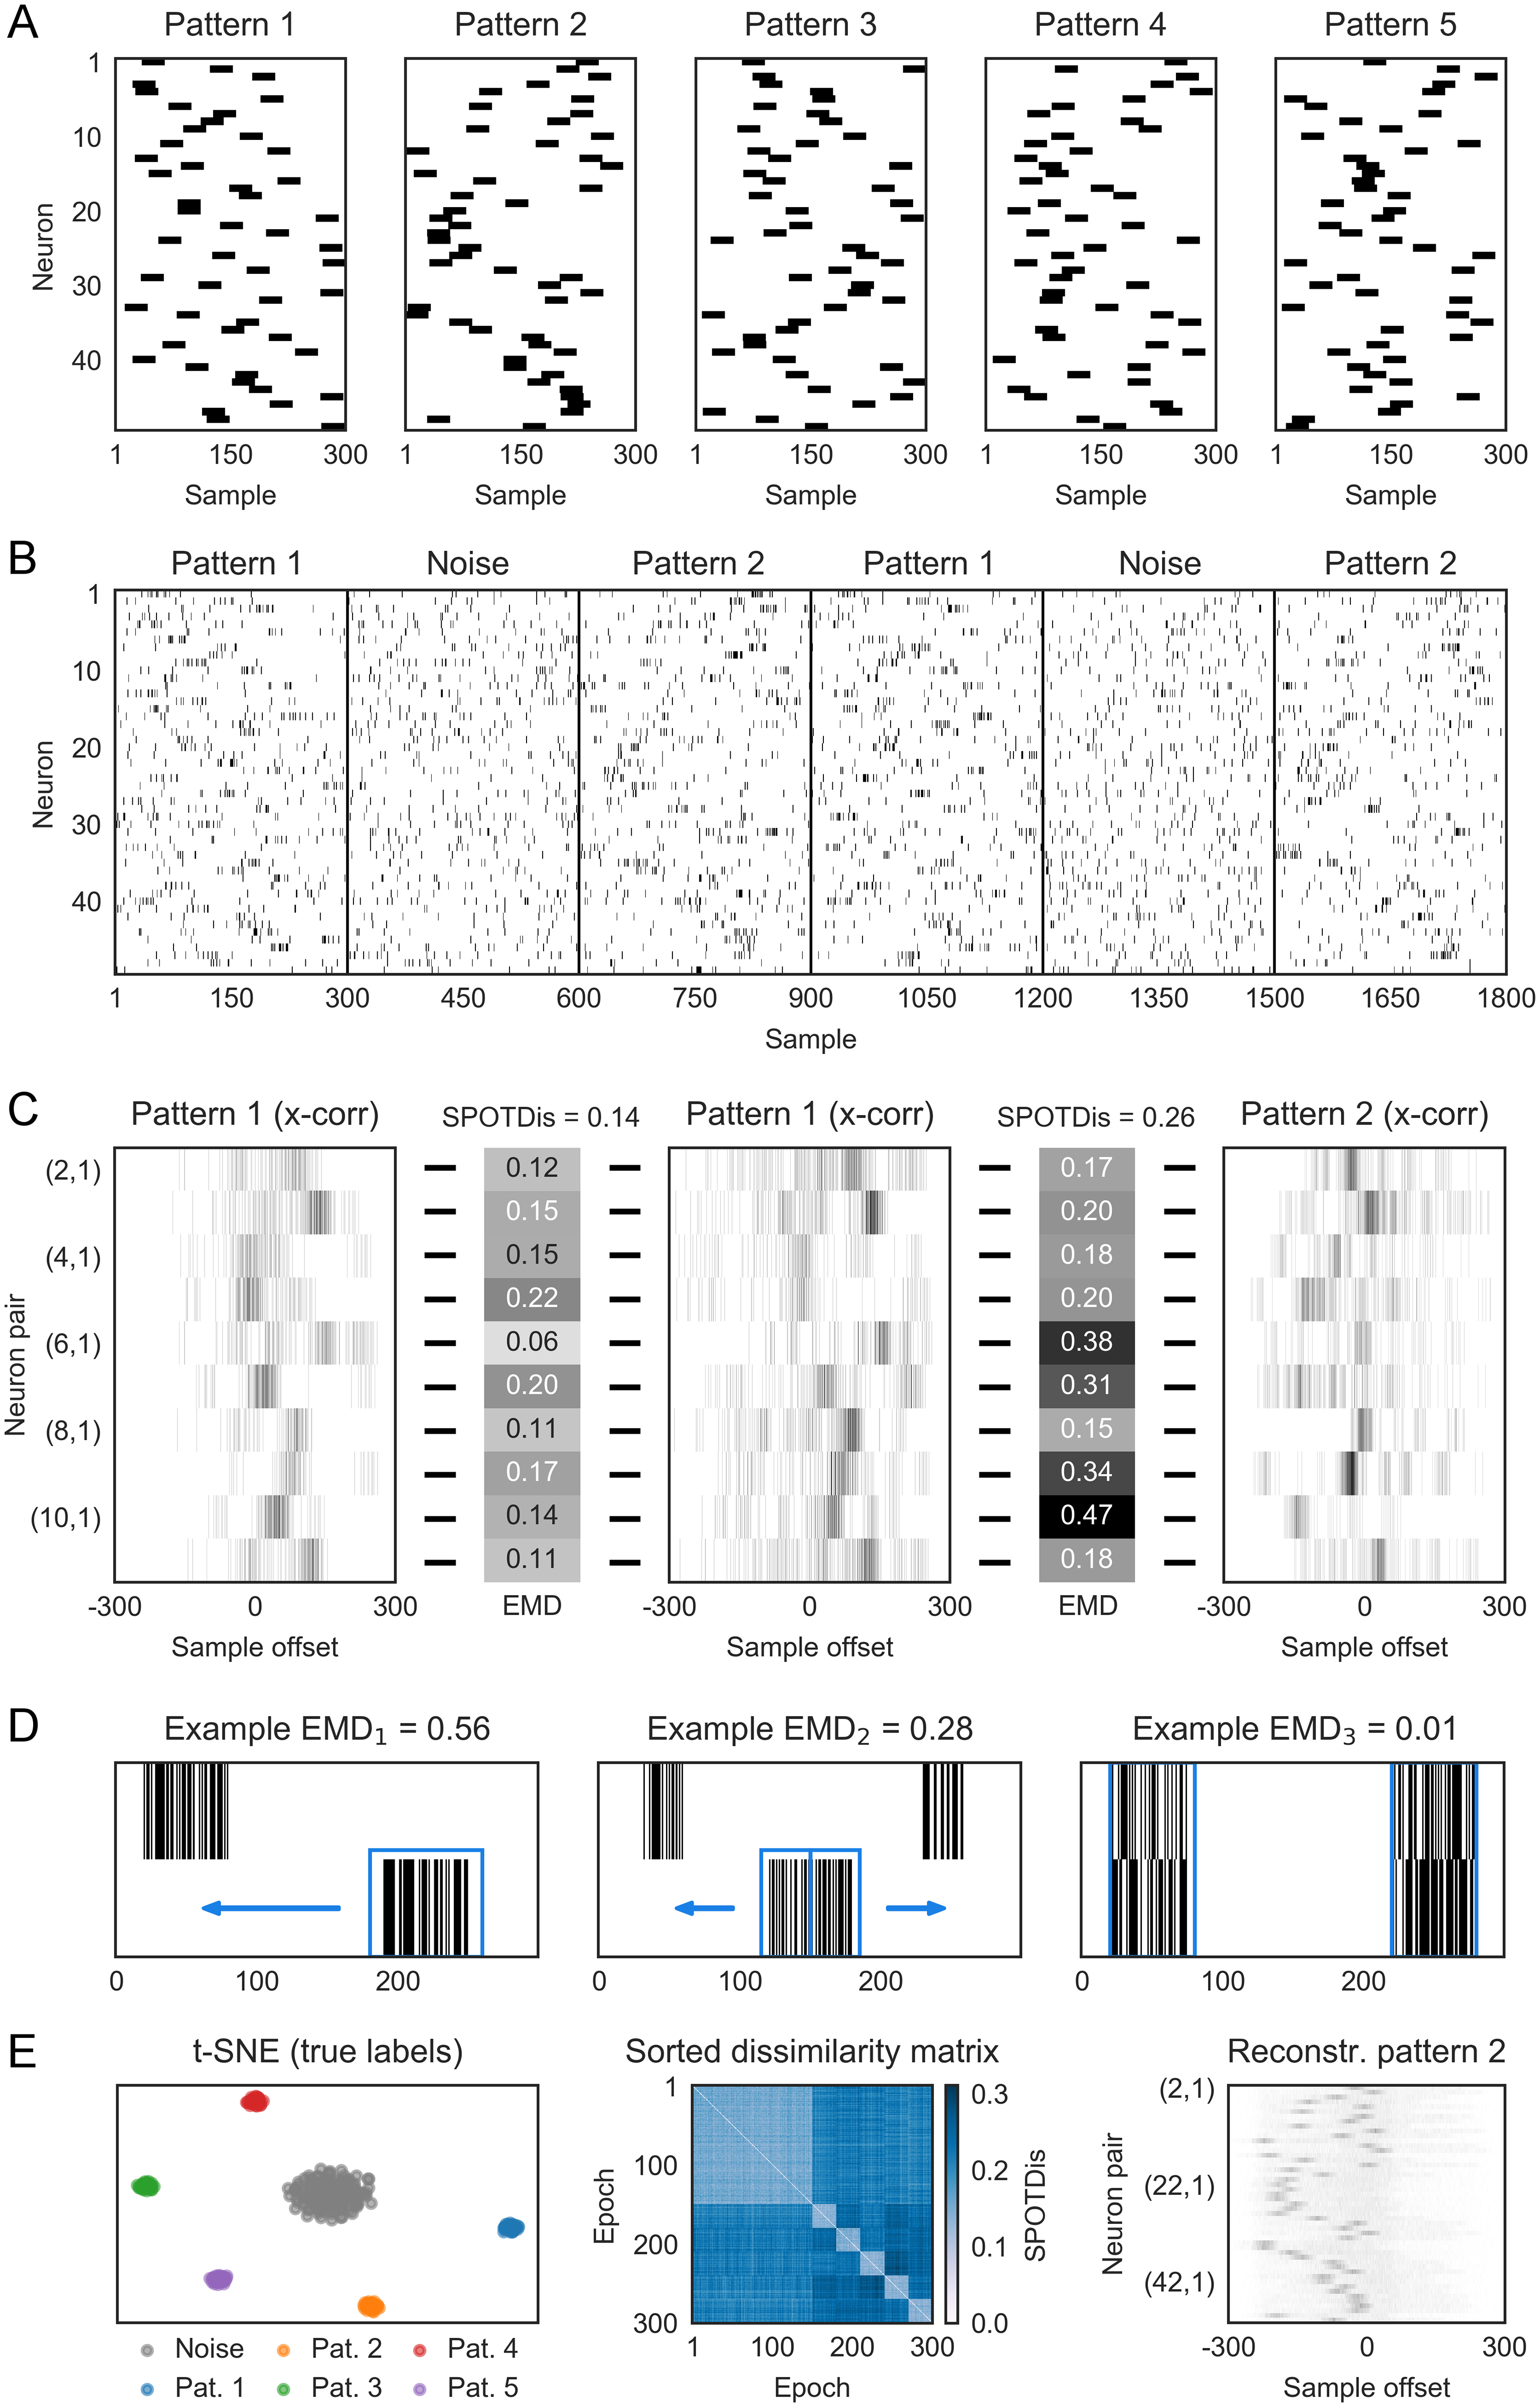
\includegraphics[width=7in,height=\textheight]{images/pcbi.1006283.g001.PNG_L.png}
\caption{Fig 1 of~\citep{grossberger_unsupervised_2018}: ``Simulated example illustrating the steps in SPOTDisClust. A) Structure of five ``ground-truth'' patterns (\ldots). For each pattern and each neuron, a random position was chosen for the activation pulse. B) Neuronal output is generated according to an inhomogeneous Poisson process, with rates dictated by the patterns in (A)." (© Authors under a \href{https://journals.plos.org/ploscompbiol/article?id=10.1371/journal.pcbi.1006283}{CC licence})}\label{fig:G2018-1}
\end{figure}

\begin{itemize}
 \item
  ``However, SPOTDis has two principal weaknesses that we address here: (1) Its computational complexity, for comparing two time epochs, is O(N2), where N is the number of neurons. This becomes a major problem for computing an M dissimilarity matrix (for M time epochs) for thousands of neurons. (2) It relies exclusively on pairwise spike-timing relationships (i.e 2nd order correlations), because it does not solve the optimal transport problem for the entire spike pattern, but only for neuron pairs separately. Hence, it may not be sensitive to higher-order correlations in spiking
  patterns.
  Here, we develop a novel dissimilarity measure for multi-neuron spiking patterns called SpikeShip, which has linear computational complexity of O(N). We achieve this by (1) computing the minimum transport cost of spikes for each spike train separately, and (2) discounting a global translation term in the transport flow across neurons.''
  https://doi.org/10.1101/2020.06.03.131573;
\end{itemize}

\subsubsection{Paper by Russo et al 2017~\citep{russo_cell_2017}}\label{paper-by-russo-et-al-2017-russo2017}
\begin{itemize}
 \item
  ``Here we present such a unifying methodological and conceptual framework which detects assembly structure at many different time scales, levels of precision, and with arbitrary internal organization.'' by~\citep{russo_cell_2017}
\item
  sliding window as in~\citep{grun_unitary_2002} (``Numerous other statistical procedures for detecting assemblies or sequential patterns have been proposed previously'') - extended to multiple lags~\citep{torre_synchronous_2016}
\item
  based on a ``non-stationarity-corrected parametric test statistic for assessing the independence of pairs'' and ``an agglomerative, heuristic clustering algorithm for fusing significant pairs into higher-order assemblies''
\end{itemize}

\subsubsection{Neural Variability and Sampling-Based Probabilistic Representations in the Visual Cortex~\citep{orban_neural_2016}}\label{neural-variability-and-sampling-based-probabilistic-representations-in-the-visual-cortex-orban2016}
\begin{itemize}
 \item
  Stochastic sampling links perceptual uncertainty to neural response variability
\item
  Model accounts for independent changes in strength and variability of responses
\item
  Model predicts relationship between noise, signal, and spontaneous correlations
\item
  Stimulus statistics dependence of response statistics is explained
\end{itemize}

To overcome the limits of models which require spike times to be discretized, utilize a sub-optimal least-squares criterion, or do not provide uncertainty estimates for model predictions or estimated parameters,~\citep{williams_point_2020} address each of these shortcomings by developing a point process model that characterizes fine-scale sequences at the level of individual spikes and represents sequence occurrences as a small number of marked events in continuous time. They also introduce learnable time warping parameters to model sequences of varying duration, which have been experimentally observed in neural circuits and demonstrate these advantages on experimental recordings from songbird higher vocal center and rodent hippocampus.

\subsubsection{Dynamics of Delay-Coupled Excitable Neural Systems}\label{dynamics-of-delay-coupled-excitable-neural-systems}
uses a FPGA
~\citep{dahlem_dynamics_2009}

\begin{verbatim}
February 2009International Journal of Bifurcation and Chaos 19(02):745-753
\end{verbatim}

V. Thanasoulis, B. Vogginger, J. Partzsch and C. Mayr, ``Delay-Based Neural Computation: Pulse Routing Architecture and Benchmark Application in FPGA,'' 2021 28th IEEE International Conference on Electronics, Circuits, and Systems (ICECS), 2021, pp.~1-5
~\citep{thanasoulis_delay-based_2021}

\subsubsection{Cell assemblies at multiple time scales with arbitrary lag constellations}\label{cell-assemblies-at-multiple-time-scales-with-arbitrary-lag-constellations}
~\citep{russo_cell_2017} starts from the relatively old notion of assessing the departure of the joint spike count distribution of two units (or sets) from independence. It is based on unitary events in multiple single-neuron spiking activity~\citep{grun_unitary_2002-1} and the reliable and efficient analysis of an excess or deficiency of joint-spike events~\citep{pipa_neuroxidence_2008}. Having derived a fast, non-stationarity-corrected parametric test statistic for assessing the independence of pairs, they designed an agglomerative, heuristic clustering algorithm for fusing significant pairs into higher-order assemblies.

\section{Learning to detect polychronous groups}\label{learning-to-detect-polychronous-groups}
\subsection{Learning weights \ldots{} and delays}\label{learning-weights-and-delays}
spike time coding in a neuron: We will describe the Spike-Time Dependent Plasticity (STDP)~\citep{ref-19NyVq80B} rule which implement an unsupervised learning aiming at optimizing the detection of polychronous patterns, that is volleys of spikes which are synchronized, up to some stable pattern of pre-synaptic delays. This STDP rule will be based by the inversion of the generative model for spike formation and will therefore be derived by a Bayesian approach. This will decouple the active synapses (similarly to a logistic regression) from the values of possible synaptic delays.

\begin{itemize}
 \item
 ~\citep{perrinet_coherence_2002} : coherence detection
\item
 ~\citep{perrinet_networks_2001} : STDP
\item
  Masquelier, Gilson et al.~- 2010 - STDP in Recurrent Neuronal Networks~\citep{gilson_stdp_2010} or Delay Selection by Spike-Timing-Dependent Plasticity in Recurrent Networks of Spiking Neurons Receiving Oscillatory Inputs. PLoS Comput Biol 9(2): e1002897.~\citep{kerr_delay_2013} which targets at the selective potentiation of recurrent connections with different axonal and dendritic delays during oscillatory activity.
\end{itemize}

Our ability to track and respond to rapidly changing visual stimuli, such as a fast-moving tennis ball, indicates that the brain is capable of extrapolating the trajectory of a moving object to predict its current position, despite the delays that result from neural transmission. Here, we show how the neural circuits underlying this ability can be learned through spike-timing-dependent synaptic plasticity and that these circuits emerge spontaneously and without supervision. This demonstrates how the neural transmission delays can, in part, be compensated to implement the extrapolation mechanisms required to predict where a moving object is at the present moment.~\citep{burkitt_predictive_2021}

\textbf{TODO amelie} section sur l'apprentissage des délais dans la biologie

~\citep{nadafian_bio-plausible_2020}


Bio-plausible Unsupervised Delay Learning for Extracting Temporal Features in Spiking Neural Networks
Alireza Nadafian, Mohammad Ganjtabesh

\begin{verbatim}
The plasticity of the conduction delay between neurons plays a fundamental role in learning. However, the exact underlying mechanisms in the brain for this modulation is still an open problem. Understanding the precise adjustment of synaptic delays could help us in developing effective brain-inspired computational models in providing aligned insights with the experimental evidence. In this paper, we propose an unsupervised biologically plausible learning rule for adjusting the synaptic delays in spiking neural networks. Then, we provided some mathematical proofs to show that our learning rule gives a neuron the ability to learn repeating spatio-temporal patterns. Furthermore, the experimental results of applying an STDP-based spiking neural network equipped with our proposed delay learning rule on Random Dot Kinematogram indicate the efficacy of the proposed delay learning rule in extracting temporal features.
\end{verbatim}

Integrating synaptic delay plasticity into supervised learning and proposes a novel learning method that adjusts both the synaptic delays and weights of the learning neurons to make them fire precisely timed spikes, that is referred to as synaptic delay-weight plasticity~\citep{zhang_supervised_2020}. Uses synthetic data to extend the existing Remote Supervised Method (ReSuMe) method.

In a recent paper~\citep{ref-B493Fl4K}, authors propose a gradient descent-based learning algorithm for synaptic delays to enhance the sequential learning performance of single spiking neuron. In this algorithm, information is encoded in the relative timing of individual neuronal spikes, and learning is performed based on the exact derivatives of the postsynaptic spike times with respect to presynaptic spike times.

In a computational model, authors show that the frequently activated polychronous neuronal groups can be learned by readout neurons with joint weight-delay spike-timing-dependent plasticity~\citep{sun_learning_2016}. This uses a joint Weight-Delay Spike-Timing-Dependent Plasticity and show aan efficient learning of polychronous groups.

\subsection{Learning sequences}\label{learning-sequences}
In~\citep{duffy_variation_2019}, authors present a model to ``show a way by which the nervous system maintains precise, stereotyped behavior in the face of environmental and neural changes.'' It is shown in bridsong generation that ``A precise, temporally sparse sequence from the premotor nucleus HVC is crucial to the performance of song in songbirds''~\citep{suthers_motor_2002,wild_descending_1993,yu_temporal_1996} and this model shows how one could vary HVC activity using something similar to dropout in ML. Using such controlled variability, ``behaviors are made more robust to environmental change by continually seeking subtly new ways of performing the same task.'' Not sure however how important it is that the HVC pattern should be sparse (and similar to PGs).

\begin{itemize}
\item
  in~\citep{agus_rapid_2010}, there are ``good'' and ``bad'' noises show that some patterns are more easy to disentangle - similar to bird songs and ecological niche.
\item
  In Bellec~\citep{bellec_fitting_2021}, authors fit summary statistics of neural data with a differentiable spiking network simulator.

  \begin{itemize}
     \item
    the loss function is the cross entropy (following Bernouilli hypothesis with a GLM where each unit is modelled with a SRM neuron~\citep{gerstner_time_1995} with recurrent dynamics)
  \item
    sample and measure method to include latent / hidden neurons
  \item
    comes with code https://github.com/EPFL-LCN/pub-bellec-wang-2021-sample-and-measure
  \item
    V1-dataset : The dataset we used was collected by Smith and Kohn 49{and is publicly available at:
    http://crcns.org/data-sets/vc/pvc-11 - it is in a sense supervised with the input being the movie and the output the spikes recorded.
  \end{itemize}
\end{itemize}

A recent work~\citep{ghosh_spatiotemporal_2019} proposes a two-stage unsupervised-supervised system for the categorization of spatiotemporal actions from an event-based stream. The first stage learns spatiotemporal convolutional filters targeted to minimize event-removal related changes to a local spatiotemporal spike-event pattern. The second stage takes the output of the spatiotemporal filters as an input example containing multiple feature channels, and proceeds to train a classifier for recognition of spatiotemporal activity. For testing the system, two datasets are considered: DVS Gesture and a new action recognition dataset recorded for this work. Results demonstrate the ability of the system to outperform the state-of-the-art in event-based gesture recognition, along with demonstrating superior performance to other alternative ways of obtaining the first stage filters. Showing the potential of such representation

\subsection{TODO: more bib to read}\label{todo-more-bib-to-read}
Learning compositional sequences with multiple time scales through a hierarchical network of spiking neurons.
Maes A, Barahona M, Clopath C.PLoS Comput Biol. 2021

Characteristics of sequential activity in networks with temporally asymmetric Hebbian learning.
Gillett M, Pereira U, Brunel N.Proc Natl Acad Sci U S A. 2020

Unsupervised Learning of Persistent and Sequential Activity.
Pereira U, Brunel N.Front Comput Neurosci. 2020

From space to time: Spatial inhomogeneities lead to the emergence of spatiotemporal sequences in spiking neuronal networks.
Spreizer S, Aertsen A, Kumar A.PLoS Comput Biol. 2019

Fast and flexible sequence induction in spiking neural networks via rapid excitability changes.
Pang R, Fairhall AL.Elife. 2019 May~\citep{pang_fast_2019}

Emergence of spontaneous assembly activity in developing neural networks without afferent input.
Triplett MA, Avitan L, Goodhill GJ.PLoS Comput Biol. 2018

Training and Spontaneous Reinforcement of Neuronal Assemblies by Spike Timing Plasticity.
Ocker GK, Doiron B.Cereb Cortex. 2019.

\textbf{TODO}

\subsection{learning pattern detection on natural images / event-based cameras}\label{learning-pattern-detection-on-natural-images-event-based-cameras}
\subsubsection{sparse coding on spatio-temporal data}\label{sparse-coding-on-spatio-temporal-data}
\subsubsection{HOTS}\label{hots}
\subsubsection{Grimaldi CBMI / PAMI}\label{grimaldi-cbmi-pami}
\section{Discussion}\label{discussion}
\textbf{TODO}

\subsection{dynamical models}\label{dynamical-models}
Dumas and colleagues~\citep{panahi_generative_2021} : three levels / fourth paradigm~\citep{tolle_fourth_2011} i.e., data exploration in which the scientific models are fit to the data by learning algorithms.

\subsection{our model}\label{our-model}
Here, we develop a model for the efficient detection of such PGs based on the inversion of a probabilistic model defining the generation of the raster plot as a combination of such groups. We show that such an inference can be achieved by a neural-like computation that could itself be used as a spiking neuron, as can be implemented in a neuromorphic chip for instance. A first result is to show the efficiency of such a scheme in detecting different PGs occurring at specific times in synthetic data. The representational capacity of the PGs is particularly interesting compared to traditional models of neuronal encoding using spiking frequency. Our second result is to propose a novel learning method for learning PGs in raster plots in a self-supervised manner. Finally we demonstrate the use of this algorithm to the output of an event-based camera and how this may separate independent components from the stream of events. This end-to-end event-based computational brick could help improve the performance of current Spiking Neural Network solution currently used in neuromorphic chips.

Emergence of electronic architectures specialized in Sparse Event-Based Convolutions~\citep{di_mauro_alfio_sne_2022} or of sparsity aware algorithms~\citep{yin_sata_2022}.

and oscillations? Journal Article • DOI: 10.1007/BF00202899 Coherent oscillations: A mechanism of feature linking in the visual cortex?

\section{development}\label{development}
scaffolding of neural assemblies / existence of critical periods :~\citep{dard_rapid_2021}

%
%The introduction should briefly place the study in a broad context and highlight why it is important. It should define the purpose of the work and its significance. The current state of the research field should be reviewed carefully and key publications cited. Please highlight controversial and diverging hypotheses when necessary. Finally, briefly mention the main aim of the work and highlight the principal conclusions. As far as possible, please keep the introduction comprehensible to scientists outside your particular field of research. Citing a journal paper \cite{ref-journal}. Now citing a book reference \cite{ref-book1,ref-book2} or other reference types \cite{ref-unpublish,ref-communication,ref-proceeding}. Please use the command \citep{ref-thesis,ref-url} for the following MDPI journals, which use author--date citation: Administrative Sciences, Arts, Econometrics, Economies, Genealogy, Humanities, IJFS, Journal of Intelligence, Journalism and Media, JRFM, Languages, Laws, Religions, Risks, Social Sciences, Literature.
%%%%%%%%%%%%%%%%%%%%%%%%%%%%%%%%%%%%%%%%%%%
%\section{Materials and Methods}
%
%Materials and Methods should be described with sufficient details to allow others to replicate and build on published results. Please note that publication of your manuscript implicates that you must make all materials, data, computer code, and protocols associated with the publication available to readers. Please disclose at the submission stage any restrictions on the availability of materials or information. New methods and protocols should be described in detail while well-established methods can be briefly described and appropriately cited.
%
%Research manuscripts reporting large datasets that are deposited in a publicly avail-able database should specify where the data have been deposited and provide the relevant accession numbers. If the accession numbers have not yet been obtained at the time of submission, please state that they will be provided during review. They must be provided prior to publication.
%
%Interventionary studies involving animals or humans, and other studies require ethical approval must list the authority that provided approval and the corresponding ethical approval code.
%\begin{quote}
%This is an example of a quote.
%\end{quote}
%
%%%%%%%%%%%%%%%%%%%%%%%%%%%%%%%%%%%%%%%%%%%
%\section{Results}
%
%This section may be divided by subheadings. It should provide a concise and precise description of the experimental results, their interpretation as well as the experimental conclusions that can be drawn.
%\section{Subsection}
%\subsection{Subsubsection}
%
%Bulleted lists look like this:
%\begin{itemize}
%\item	First bullet;
%\item	Second bullet;
%\item	Third bullet.
%\end{itemize}
%
%Numbered lists can be added as follows:
%\begin{enumerate}
%\item	First item; 
%\item	Second item;
%\item	Third item.
%\end{enumerate}
%
%The text continues here. 
%
%\section{Figures, Tables and Schemes}
%
%All figures and tables should be cited in the main text as Figure~\ref{fig1}, Table~\ref{tab1}, Table~\ref{tab2}, etc.
%
%\begin{figure}[H]
%
\includegraphics[width=10.5 cm]{Definitions/logo-mdpi}
%\caption{This is a figure. Schemes follow the same formatting. If there are multiple panels, they should be listed as: (\textbf{a}) Description of what is contained in the first panel. (\textbf{b}) Description of what is contained in the second panel. Figures should be placed in the main text near to the first time they are cited. A caption on a single line should be centered.\label{fig1}}
%\end{figure}   
%\unskip
%
%\begin{table}[H] 
%\caption{This is a table caption. Tables should be placed in the main text near to the first time they are~cited.\label{tab1}}
%\newcolumntype{C}{>{\centering\arraybackslash}X}
%\begin{tabularx}{\textwidth}{CCC}
%\toprule
%\textbf{Title 1}	& \textbf{Title 2}	& \textbf{Title 3}\\
%\midrule
%Entry 1		& Data			& Data\\
%Entry 2		& Data			& Data\\
%\bottomrule
%\end{tabularx}
%\end{table}
%\unskip
%
%\begin{table}[H]
%\caption{This is a wide table.\label{tab2}}
%	\begin{adjustwidth}{-\extralength}{0cm}
%		\newcolumntype{C}{>{\centering\arraybackslash}X}
%		\begin{tabularx}{\fulllength}{CCCC}
%			\toprule
%			\textbf{Title 1}	& \textbf{Title 2}	& \textbf{Title 3}     & \textbf{Title 4}\\
%			\midrule
%			Entry 1		& Data			& Data			& Data\\
%			Entry 2		& Data			& Data			& Data \textsuperscript{1}\\
%			\bottomrule
%		\end{tabularx}
%	\end{adjustwidth}
%	\noindent{\footnotesize{\textsuperscript{1} This is a table footnote.}}
%\end{table}
%
%%\begin{listing}[H]
%%\caption{Title of the listing}
%%\rule{\columnwidth}{1pt}
%%\raggedright Text of the listing. In font size footnotesize, small, or normalsize. Preferred format: left aligned and single spaced. Preferred border format: top border line and bottom border line.
%%\rule{\columnwidth}{1pt}
%%\end{listing}
%
%Text.
%
%Text.
%
%\section{Formatting of Mathematical Components}
%
%This is the example 1 of equation:
%\begin{linenomath}
%\begin{equation}
%a = 1,
%\end{equation}
%\end{linenomath}
%the text following an equation need not be a new paragraph. Please punctuate equations as regular text.
%%% If the documentclass option "submit" is chosen, please insert a blank line before and after any math environment (equation and eqnarray environments). This ensures correct linenumbering. The blank line should be removed when the documentclass option is changed to "accept" because the text following an equation should not be a new paragraph.
%
%This is the example 2 of equation:
%\begin{adjustwidth}{-\extralength}{0cm}
%\begin{equation}
%a = b + c + d + e + f + g + h + i + j + k + l + m + n + o + p + q + r + s + t + u + v + w + x + y + z
%\end{equation}
%\end{adjustwidth}
%
%% Example of a page in landscape format (with table and table footnote).
%%\startlandscape
%%\begin{table}[H] %% Table in wide page
%%\caption{This is a very wide table.\label{tab3}}
%%	\begin{tabularx}{\textwidth}{CCCC}
%%		\toprule
%%		\textbf{Title 1}	& \textbf{Title 2}	& \textbf{Title 3}	& \textbf{Title 4}\\
%%		\midrule
%%		Entry 1		& Data			& Data			& This cell has some longer content that runs over two lines.\\
%%		Entry 2		& Data			& Data			& Data\textsuperscript{1}\\
%%		\bottomrule
%%	\end{tabularx}
%%	\begin{adjustwidth}{+\extralength}{0cm}
%%		\noindent\footnotesize{\textsuperscript{1} This is a table footnote.}
%%	\end{adjustwidth}
%%\end{table}
%%\finishlandscape
%
%% Example of a figure that spans the whole page width. The same concept works for tables, too.
%\begin{figure}[H]
%\begin{adjustwidth}{-\extralength}{0cm}
%\centering
%
\includegraphics[width=13.5cm]{Definitions/logo-mdpi}
%\end{adjustwidth}
%\caption{This is a wide figure.\label{fig2}}
%\end{figure}  
%
%Please punctuate equations as regular text. Theorem-type environments (including propositions, lemmas, corollaries etc.) can be formatted as follows:
%%% Example of a theorem:
%\begin{Theorem}
%Example text of a theorem.
%\end{Theorem}
%
%The text continues here. Proofs must be formatted as follows:
%
%%% Example of a proof:
%\begin{proof}[Proof of Theorem 1]
%Text of the proof. Note that the phrase ``of Theorem 1'' is optional if it is clear which theorem is being referred to.
%\end{proof}
%The text continues here.
%
%%%%%%%%%%%%%%%%%%%%%%%%%%%%%%%%%%%%%%%%%%%
%\section{Discussion}
%
%Authors should discuss the results and how they can be interpreted from the perspective of previous studies and of the working hypotheses. The findings and their implications should be discussed in the broadest context possible. Future research directions may also be highlighted.
%
%%%%%%%%%%%%%%%%%%%%%%%%%%%%%%%%%%%%%%%%%%%
%\section{Conclusions}
%
%This section is not mandatory, but can be added to the manuscript if the discussion is unusually long or complex.

%%%%%%%%%%%%%%%%%%%%%%%%%%%%%%%%%%%%%%%%%%
%%%%%%%%%%%%%%%%%%%%%%%%%%%%%%%%%%%%%%%%%%
\vspace{6pt} 

%%%%%%%%%%%%%%%%%%%%%%%%%%%%%%%%%%%%%%%%%%
%% optional
%\supplementary{The following supporting information can be downloaded at:  \linksupplementary{s1}, Figure S1: title; Table S1: title; Video S1: title.}

% Only for the journal Methods and Protocols:
% If you wish to submit a video article, please do so with any other supplementary material.
% \supplementary{The following supporting information can be downloaded at: \linksupplementary{s1}, Figure S1: title; Table S1: title; Video S1: title. A supporting video article is available at doi: link.}

%%%%%%%%%%%%%%%%%%%%%%%%%%%%%%%%%%%%%%%%%%
\authorcontributions{For research articles with several authors, a short paragraph specifying their individual contributions must be provided. The following statements should be used ``Conceptualization, X.X. and Y.Y.; methodology, X.X.; software, X.X.; validation, X.X., Y.Y. and Z.Z.; formal analysis, X.X.; investigation, X.X.; resources, X.X.; data curation, X.X.; writing---original draft preparation, X.X.; writing---review and editing, X.X.; visualization, X.X.; supervision, X.X.; project administration, X.X.; funding acquisition, Y.Y. All authors have read and agreed to the published version of the manuscript.'', please turn to the  \href{http://img.mdpi.org/data/contributor-role-instruction.pdf}{CRediT taxonomy} for the term explanation. Authorship must be limited to those who have contributed substantially to the work~reported.}

\funding{Please add: ``This research received no external funding'' or ``This research was funded by NAME OF FUNDER grant number XXX.'' and  and ``The APC was funded by XXX''. Check carefully that the details given are accurate and use the standard spelling of funding agency names at \url{https://search.crossref.org/funding}, any errors may affect your future funding.}

\institutionalreview{In this section, you should add the Institutional Review Board Statement and approval number, if relevant to your study. You might choose to exclude this statement if the study did not require ethical approval. Please note that the Editorial Office might ask you for further information. Please add “The study was conducted in accordance with the Declaration of Helsinki, and approved by the Institutional Review Board (or Ethics Committee) of NAME OF INSTITUTE (protocol code XXX and date of approval).” for studies involving humans. OR “The animal study protocol was approved by the Institutional Review Board (or Ethics Committee) of NAME OF INSTITUTE (protocol code XXX and date of approval).” for studies involving animals. OR “Ethical review and approval were waived for this study due to REASON (please provide a detailed justification).” OR “Not applicable” for studies not involving humans or animals.}

\informedconsent{Any research article describing a study involving humans should contain this statement. Please add ``Informed consent was obtained from all subjects involved in the study.'' OR ``Patient consent was waived due to REASON (please provide a detailed justification).'' OR ``Not applicable'' for studies not involving humans. You might also choose to exclude this statement if the study did not involve humans.

Written informed consent for publication must be obtained from participating patients who can be identified (including by the patients themselves). Please state ``Written informed consent has been obtained from the patient(s) to publish this paper'' if applicable.}

\dataavailability{
%This works is made reproducible using the following tools. First the code reproducing all figures is available on \href{https://github.com/SpikeAI/2022-09_UltraFastCat/blob/main/Readme.md}{GitHub}~\citep{Jeremie2022a}.

%\noindent The paper is available a an \href{https://arxiv.org/abs/2205.03635}{arXiv preprint} with links to previous versions ands to the code. 
Find the associated \noindent \href{https://www.zotero.org/groups/4562620/polychronies}{zotero group} used to regroup relevant literature on the subject.

} 

\acknowledgments{In this section you can acknowledge any support given which is not covered by the author contribution or funding sections. This may include administrative and technical support, or donations in kind (e.g., materials used for experiments).}

\conflictsofinterest{Declare conflicts of interest or state ``The authors declare no conflict of interest.'' Authors must identify and declare any personal circumstances or interest that may be perceived as inappropriately influencing the representation or interpretation of reported research results. Any role of the funders in the design of the study; in the collection, analyses or interpretation of data; in the writing of the manuscript; or in the decision to publish the results must be declared in this section. If there is no role, please state ``The funders had no role in the design of the study; in the collection, analyses, or interpretation of data; in the writing of the manuscript; or in the decision to publish the~results''.} 

%%%%%%%%%%%%%%%%%%%%%%%%%%%%%%%%%%%%%%%%%%
%% Optional
\sampleavailability{Samples of the compounds ... are available from the authors.}

%% Only for journal Encyclopedia
%\entrylink{The Link to this entry published on the encyclopedia platform.}

\abbreviations{Abbreviations}{
The following abbreviations are used in this manuscript:\\

\noindent 
\begin{tabular}{@{}ll}
MDPI & Multidisciplinary Digital Publishing Institute\\
DOAJ & Directory of open access journals\\
TLA & Three letter acronym\\
LD & Linear dichroism
\end{tabular}
}

%%%%%%%%%%%%%%%%%%%%%%%%%%%%%%%%%%%%%%%%%%
%% Optional
\appendixtitles{no} % Leave argument "no" if all appendix headings stay EMPTY (then no dot is printed after "Appendix A"). If the appendix sections contain a heading then change the argument to "yes".
\appendixstart
\appendix
\section[\appendixname~\thesection]{}
\subsection[\appendixname~\thesubsection]{}
The appendix is an optional section that can contain details and data supplemental to the main text---for example, explanations of experimental details that would disrupt the flow of the main text but nonetheless remain crucial to understanding and reproducing the research shown; figures of replicates for experiments of which representative data are shown in the main text can be added here if brief, or as Supplementary Data. Mathematical proofs of results not central to the paper can be added as an appendix.

\begin{table}[H] 
\caption{This is a table caption.\label{tab5}}
\newcolumntype{C}{>{\centering\arraybackslash}X}
\begin{tabularx}{\textwidth}{CCC}
\toprule
\textbf{Title 1}	& \textbf{Title 2}	& \textbf{Title 3}\\
\midrule
Entry 1		& Data			& Data\\
Entry 2		& Data			& Data\\
\bottomrule
\end{tabularx}
\end{table}

\section[\appendixname~\thesection]{}
All appendix sections must be cited in the main text. In the appendices, Figures, Tables, etc. should be labeled, starting with ``A''---e.g., Figure A1, Figure A2, etc.

%%%%%%%%%%%%%%%%%%%%%%%%%%%%%%%%%%%%%%%%%%

%%%%%%%%%%%%%%%%%%%%%%%%%%%%%%%%%%%%%%%%%%
\begin{adjustwidth}{-\extralength}{0cm}
%\printendnotes[custom] % Un-comment to print a list of endnotes

%%%%%%%%% REFERENCES
\reftitle{References}

% Please provide either the correct journal abbreviation (e.g. according to the “List of Title Word Abbreviations” http://www.issn.org/services/online-services/access-to-the-ltwa/) or the full name of the journal.
% Citations and References in Supplementary files are permitted provided that they also appear in the reference list here. 

\bibliography{references}

%\begin{thebibliography}{00}
%\printbibliography[heading=none]
%\end{thebibliography}

% For the MDPI journals use author-date citation, please follow the formatting guidelines on http://www.mdpi.com/authors/references
% To cite two works by the same author: \citeauthor{ref-journal-1a} (\citeyear{ref-journal-1a}, \citeyear{ref-journal-1b}). This produces: Whittaker (1967, 1975)
% To cite two works by the same author with specific pages: \citeauthor{ref-journal-3a} (\citeyear{ref-journal-3a}, p. 328; \citeyear{ref-journal-3b}, p.475). This produces: Wong (1999, p. 328; 2000, p. 475)

\end{adjustwidth}
\end{document}

